\documentclass[twoside]{article}
\setlength{\oddsidemargin}{0.25 in}
\setlength{\evensidemargin}{-0.25 in}
\setlength{\topmargin}{-0.6 in}
\setlength{\textwidth}{6.5 in}
\setlength{\textheight}{8.5 in}
\setlength{\headsep}{0.75 in}
\setlength{\parindent}{0 in}
\setlength{\parskip}{0.1 in}

%
% ADD PACKAGES here:
%

\usepackage{amsmath,amsfonts,amssymb,graphicx,mathtools,flexisym, hyperref, enumerate,mathtools,tikz}
\usetikzlibrary{arrows}

%
% The following commands set up the lecnum (lecture number)
% counter and make various numbering schemes work relative
% to the lecture number.
%
\newcounter{lecnum}
\renewcommand{\thepage}{\thelecnum-\arabic{page}}
\renewcommand{\thesection}{\thelecnum.\arabic{section}}
\renewcommand{\theequation}{\thelecnum.\arabic{equation}}
\renewcommand{\thefigure}{\thelecnum.\arabic{figure}}
\renewcommand{\thetable}{\thelecnum.\arabic{table}}

%
% The following macro is used to generate the header.
%
\newcommand{\lecture}[4]{
   \pagestyle{myheadings}
   \thispagestyle{plain}
   \newpage
   \setcounter{lecnum}{#1}
   \setcounter{page}{1}
   \noindent
   \begin{center}
   \framebox{
      \vbox{\vspace{2mm}
    \hbox to 6.28in { {\bf MATH2923: Advance Analysis
    \hfill } }
       \vspace{4mm}
       \hbox to 6.28in { {\Large \hfill #1. #2 \hfill} }
       \vspace{4mm}
       }
   }
   \end{center}
}
%
% Convention for citations is authors' initials followed by the year.
% For example, to cite a paper by Leighton and Maggs you would type
% \cite{LM89}, and to cite a paper by Strassen you would type \cite{S69}.
% (To avoid bibliography problems, for now we redefine the \cite command.)
% Also commands that create a suitable format for the reference list.
\renewcommand{\cite}[1]{[#1]}
\def\beginrefs{\begin{list}%
        {[\arabic{equation}]}{\usecounter{equation}
         \setlength{\leftmargin}{2.0truecm}\setlength{\labelsep}{0.4truecm}%
         \setlength{\labelwidth}{1.6truecm}}}
\def\endrefs{\end{list}}
\def\bibentry#1{\item[\hbox{[#1]}]}

\newcommand{\Lim}[1]{\raisebox{0.5ex}{\scalebox{0.8}{$\displaystyle \lim_{#1}\;$}}}
\newcommand{\Inf}[1]{\raisebox{0.5ex}{\scalebox{0.8}{$\displaystyle \inf_{#1}\;$}}}
\newcommand{\Sup}[1]{\raisebox{0.5ex}{\scalebox{0.8}{$\displaystyle \sup_{#1}\;$}}}
\newcommand{\norm}[1]{\left\lVert#1\right\rVert}

%Use this command for a figure; it puts a figure in wherever you want it.
%usage: \fig{NUMBER}{SPACE-IN-INCHES}{CAPTION}
\newcommand{\fig}[3]{
            \vspace{#2}
            \begin{center}
            Figure \thelecnum.#1:~#3
            \end{center}
    }
% Use these for theorems, lemmas, proofs, etc.
\newtheorem{theorem}{Theorem}[lecnum]
\newtheorem{lemma}[theorem]{Lemma}
\newtheorem{proposition}[theorem]{Proposition}
\newtheorem{claim}[theorem]{Claim}
\newtheorem{axiom}[theorem]{Axiom}
\newtheorem{remark}[theorem]{Remark}
\newtheorem{corollary}[theorem]{Corollary}
\newtheorem{example}[theorem]{Example}
\newtheorem{definition}[theorem]{Definition}
\newenvironment{proof}{{\bf Proof:}}{\hfill\rule{2mm}{2mm}}


%
% To generate a clickable table of content.
%
\hypersetup{
    colorlinks,
    citecolor=black,
    filecolor=black,
    linkcolor=blue,
    urlcolor=black
}


\newcommand\E{\mathbb{E}}
\newcommand{\seq}{\{x_n\}_{n \geq 0}}

\usepackage{tocloft}

\addtolength{\cftsecnumwidth}{10pt}
\setlength{\cftsubsecnumwidth}{3.5em}
\setlength{\cftsubsubsecnumwidth}{4.5em}



\title{MATH2923: Advance Analysis}
\author{Charles Christopher Hyland}
\date{Semester 2 2018}


\begin{document}

\pagenumbering{gobble}
\maketitle
\begin{abstract}
Thank you for stopping by to read this. These are notes collated from lectures and tutorials as I took this course.
\end{abstract}
\newpage
\tableofcontents
\newpage
\pagenumbering{arabic}

%\lecture{**CHAPTER-NUMBER**}{**TITLE**}
\lecture{1}{Axioms and Bounds}
\section{Foundations and Axioms}
\section{Foundations and Axioms}
\subsection{Axioms}

\begin{axiom}
(Peano Axioms for $\mathbb{N}$). The set of natural numbers is a set $\mathbb{N}$ with a distinguished element 0 and a successor function S that is
\begin{enumerate}
  \item S: $\mathbb{N} \rightarrow \mathbb{N}$/{0} is injective.
  \item If 0 $\in$ N and S(n) $\in$ N $\forall n \in \mathbb{N}$, then N = $\mathbb{N}$.
\end{enumerate}
\end{axiom}

\begin{definition}
(Rational Numbers). The set of $\textit{rational numbers } \mathbb{Q}$ is the set \{$\frac{p}{q}$: p, q $\in \mathbb{Z}$\}.
\end{definition}

\begin{definition}
(Group). A $\textit{group}$ (G, .) is a set with a binary operator . (such as the addition operator) defined on it. It satisfies the 4 group axioms:
\begin{enumerate}
  \item Closure: For all a, b in G, a . b $\in$ G.
  \item Associative: For all a, b in G, (a . b) . c = a . (b . c).
  \item Identity Element: There is an identity element e such that e . a = a.
  \item Inverse Element: For all a in G, there exist an inverse element a' such that a.a' = e.
\end{enumerate} 
\end{definition}

\begin{remark}
A group is referred to as $\textit{abelian}$ if a . b = b . a 
\end{remark}

\begin{remark}
A $\textit{monoid}$ is a group without the property of inverse elements.
\end{remark}

\begin{definition}
(Integers $\mathbb{Z}$). The set of integers $\mathbb{Z}$ with the addition (+) and multiplication (.) binary operator defined on it ($\mathbb{Z}$, +, .) is an $\mathit{abelian}$ group under addition ($\mathbb{Z}$, +) and a $\mathit{monoid}$ under multiplication ($\mathbb{Z}$, .). The multiplication operator is distributive with respect to addition.
\end{definition}

\begin{definition}
(Field). A $\textit{field}$ is a set with 2 operations addition and multiplication such that the it is an $\textit{abelian}$ group under addition, an $\textit{abelian}$ group under multiplication for nonzero elements, and the multiplication is distributive over addition.
\end{definition}

\begin{remark}
The set of rational numbers $\mathbb{Q}$ and real numbers $\mathbb{R}$ forms a field.
\end{remark}

We now seek to derive the properties of $\mathbb{R}$ from the 3 axioms: field, order, and completeness.

\begin{axiom}
(Field Axioms). The $\textit{field}$ axioms are the properties of a field as defined earlier.
\end{axiom}

We now establish the notion of $\textit{order}$ in a set.
\begin{axiom}
(Order Axioms). There exists a relation $<$ on $\mathbb{R}$ with the following 4 properties.
\begin{enumerate}
  \item x $<$ y iff 0 $<$ y - x;
  \item If 0 $<$ x,y then 0 $<$ x + y;
  \item If 0 $<$ x,y then 0 $<$ xy;
  \item For every $x \in \mathbb{R}$, either 0 $<$ -x,  0 $<$ x, or x = 0.
\end{enumerate}
\end{axiom}
\begin{remark}
Note that we only used the $<$ operator since that is the only thing that has been defined so far.
\end{remark}

\begin{remark}
What we have now constructed are $\textbf{partially ordered sets}$. Note that this is different to $\textbf{total order sets}$, which are sets that require every element of the set to be comparable to one another.
\end{remark}

\subsection{Boundedness}

Before we define the $\textit{completeness}$ axiom, we need to define some other things first.

\begin{definition}
(Upper and Lower Bounds). The set A $\subseteq \mathbb{R}$ is $\textit{bounded}$ from above (below) if there exists m $\in \mathbb{R}$ such that $x \leq m$ ($x \geq m$) for all $x \in A$. Every m that satisfies this property is known as an $\textit{upper bound}$ ($\textit{lower bound}$) of A. 
\end{definition}

\begin{definition}
(Bounded). A set is $\textit{bounded}$ if it is bounded from above $\textbf{and}$ bounded from below.
\end{definition}

\begin{definition}
(Supremum). Let A $\subseteq \mathbb{R}$ be a subset bounded from above and is $\textbf{non-empty}$. We say that M $\in \mathbb{R}$ is a $\textit{supremum}$ of A if it satisfies the $\textbf{two}$ conditions that
\begin{enumerate}[(i)]
  \item M is an upper bound of A;
  \item $M \leq m$ for every upper bound m of A. 
\end{enumerate}
\end{definition}

\begin{definition}
(Infimum). Let A $\subseteq \mathbb{R}$ be a subset bounded from below and is $\textbf{non-empty}$. We say that N $\in \mathbb{R}$ is a $\textit{infimum}$ of A if it satisfies the $\textbf{two}$ conditions that
\begin{enumerate}[(i)]
  \item N is an lower bound of A;
  \item $N \geq n$ for every lower bound n of A. 
\end{enumerate}
\end{definition}

\begin{remark}
(Least Upper Bound and Greatest Lower Bound). We refer to the supremum (infimum) as the $\textit{least upper bound}$ ($\textit{greatest lower bound}$). An unbounded set has a supremum of $\infty$ and an infimum of -$\infty$.
\end{remark}

\begin{remark}
The supremum (infimum) of a set is $\textbf{unique}$. 
\end{remark}

\begin{definition}
(Maximum and Minimum). A supremum (infimum) that is also $\textbf{in}$ the set A is known as a $\textit{maximum}$ ($\textit{minimum}$).
\end{definition}

\begin{remark}
A maximum is $\textbf{always}$ a supremum but a supremum is not always a maximum.
\end{remark}

Collecting all this, we can now state the third axiom.

\begin{axiom}
(Least Upper Bound Axiom). Every non-empty set $A \subseteq \mathbb{R}$ which is bounded from above $\textbf{admits}$ a supremum.
\end{axiom}

Additionally, we could phrase it in terms of the $\textbf{infimum}$.

\begin{axiom}
(Greatest Lower Bound Axiom). Every non-empty set $A \subseteq \mathbb{R}$ which is bounded from below $\textbf{admits}$ an infimum.
\end{axiom}

\begin{remark}
The only field that satisfies all 3 axioms (field, order, and completeness) is the field of real numbers.
\end{remark}

\lecture{2}{Basic Properties of Real Numbers}
\section{Proprties of Real numbers}
\subsection{More things on Supremum and Infimum}

\begin{lemma}
Let A $\neq \emptyset$ be a subset of $\mathbb{R}$. The following assertions are true.
\begin{enumerate}[(i)]
  \item If t $<$ sup A, then there exists a $\in$ A such that t $<$ a;
  \item If t $>$ inf A, then there exists a $\in$ A such that t $>$ a;
\end{enumerate}
\end{lemma}

\begin{proof}
i) Suppose there did not exist an element a $\in$ A. Then that means t $\leq$ a for all a $\in$ A. Therefore t is a smaller upper bound than the supremum, which is a contradiction. Hence, there exists an element a $\in$ A that is greater than t.

2) Suppose there did not exist an element a $\in$ A. Then that means t $\geq$ a for all a $\in$ A. Therefore t is a larger lower bound that the infimum, which is a contradiction. Hence, there exists an element a $\in$ A that is lower than t.
\end{proof}

From the greatest lower bound axiom, it guarantees the existence of supremums for sets bounded above. We can use this axiom to show that this is equivalent to the existence of infimums for sets bounded by below.

\begin{proposition}
The following 3 statements are equivalent:
\begin{enumerate}[(i)]
  \item sup A exists for every non-empty A $\subseteq \mathbb{R}$ bounded from above.
  \item inf A exists for every non-empty A $\subseteq \mathbb{R}$ bounded from below.
  \item If A, B $\subseteq \mathbb{R}$ are sets such that $a \leq b$ for all a $\in$ A and b $\in$ B. Then there exists c $\in \mathbb{R}$ with $a \leq c \leq b$ for all $a \in A$ and $b \in B$. 
\end{enumerate}
\end{proposition}

\begin{proof}(Sketch).

(1 $\rightarrow$ 2)

Construct a set of lower bounds for $B \subseteq \mathbb{R}$. Denote this set as set A. Then show that the supremum of set A is the infimum of set B.

(2 $\rightarrow$ 3)

Let $a \leq b$ for all $a \in A, b \in B$. Then define $c \coloneqq infB$. We then need to show c is $a \leq c \leq b$ for all $a \in A$ and $b \in B$.

(3 $\rightarrow$ 1)

Construct a set of upper bounds for A and denote it as B. Then we claim that c is the supremum of A. Hence, show that c is an upper bound of A and it is the smallest element out of the set of upper bounds in B.
\end{proof}

\begin{proposition}
Let $A, B \subseteq \mathbb{R}$ such that $A \subseteq B$. This implies that $sup A \leq sup B$.
\end{proposition}
\begin{proof}
An upperbound of B is also an upperbound of A. This is true for all upperbounds of B. Hence, by definition of a supremum, $sup A \leq sup B$.
\end{proof}

\begin{proposition}
Let $A \subseteq \mathbb{R}$ and non-empty. Then
$$
sup A = -inf(-A).
$$
\end{proposition}
\begin{proof}
Look at the infimum of -A. We have that $M \coloneqq inf(-A)$. Therefore, $-M \leq -x$ for all x in A. Hence, we have that $M \geq x$ for all x in A, therefore M is an upperbound of A. Now for any lower bounds $-m \leq -x$ for all $x \in A$, we have that $m \geq x$ for all $x \in A$ but $m \geq M$ and therefore M is the supremum.
\end{proof}

\begin{proposition}
Let $A + B = \{x+y: x \in A, y \in B\}$. Then
$$
sup(A + B) = sup A + sup B.
$$
\end{proposition}

\begin{proposition}
Let $s \coloneqq sup A \not \in A$, then there exists a strictly increasing $x_n \in A$ with $sup_{n \in \mathbb{N}}x_n = s$.
\end{proposition}

\subsection{Basic Properties of the Real Numbers}

\begin{proposition}
(Archimedian Property of $\mathbb{N}$). For every x $\in \mathbb{R}$, there exists n $\in \mathbb{N}$ such that x $<$ n.
\end{proposition}

\begin{proof} (Sketch).

To prove this, use a proof by contradiction.
\end{proof}

\begin{corollary}
For every $\epsilon > 0$, there exist a $n \in \mathbb{N}$ such that:
$$
0 < \frac{1}{n} < \epsilon
$$
\end{corollary}

\begin{proof}
Using the Archimedian property by setting x as $\frac{1}{\epsilon}$,
$$
\frac{1}{\epsilon} < n
$$
We then rearrange and the proof is complete.
\end{proof}

\bigskip
We can look at the distribution of the rational and irrational numbers in $\mathbb{R}$. 

\begin{proposition}
(Density of rational and irrational numbers). Suppose that a, b $\in \mathbb{R}$ with a $<$ b. Then:
\begin{enumerate}[(i)]
  \item There exists $q \in \mathbb{Q}$ such that $a < q < b$ (The rationals are dense in $\mathbb{R}$); 
  \item There exists $i \in \mathbb{I}$ with $a < i < b$ (The irrationals $\mathbb{I}$ are dense in $\mathbb{R}$).
\end{enumerate}
\end{proposition}


We can now show that $\mathbb{Q}$ does not satisfy the least upper bound property.

\begin{proposition}
$x^2 = 2$ has no solution in $\mathbb{Q}$.
\end{proposition}

\begin{proof}
(By contradiction). Assume $x^2 = 2$ has a solution, say $\frac{p}{q}$ where p, q $\in \mathbb{Z}$ and p, q have no common factors. So: $(\frac{p}{q})^2 = 2$, hence $p^2 = 2q^2$. Then $p^2$ is $\textbf{even}$ since it is divisible by 2. Then p is even because if p was odd then $p^2$ would be odd. So p = 2m for some $m \in \mathbb{Z}$, $\rightarrow p^2 = 4m^2 = 2q^2$. Then $2m^2 = q^2$. Hence, q is even. Then this contradicts our assumption that p and q have no common factors. Therefore, $x^2 = 2$ must not have a solution.
\end{proof}

\lecture{3}{Complex Numbers and Inner Product}
\section{Complex Numbers}
\subsection{Introduction to Complex Numbers}

For every $z \in \mathbb{C}$, there exists $a, b \in \mathbb{R}$ such that:
$$
z = a + bi
$$

where we define:

\begin{enumerate}[(i)]
  \item a is known as the $\textbf{real}$ part of z;
  \item b is the $\textbf{imaginary}$ part of z;
  \item $\bar{z} = a - bi$ is the $\textbf{complex conjugate}$ of z;
  \item $|z| = \sqrt{z\bar{z}}$ = $\sqrt{a^2 + b^2} \geq 0$ is the \textbf{modulus} of z.
\end{enumerate}

The modulus of z is also known as the distance of the point (a,b) from the origin (0, 0) whilst the complex conjugate is the reflection of z on the real axis.

\begin{proposition}
  The compex numbers has the following properties:
  \begin{enumerate}[(i)]
    \item Re z = $\frac{1}{2}$(z + $\bar{z}$) and Im z = $\frac{1}{2i}$(z - $\bar{z}$);
    \item $\overline{z + w}$ = $\bar{z}$+$\bar{w}$, $\bar{zw}$ = $\bar{z}\bar{w}$, $\overline{\frac{1}{z}}$ = $\frac{1}{\bar{z}}$;
    \item $|zw| = |z||w|$ and $|z + w|$ $\leq$ $|z| + |w|$.
  \end{enumerate}
\end{proposition}

\subsection{Higher Dimensional Spaces}
We define $\mathbb{K}$ to be either $\mathbb{R}$ or $\mathbb{C}$. For $n \in \mathbb{N}$, we denote by $\mathbb{K}^n$ the set:
$$
\mathbb{K}^n = \{\mathbf{x} = (x_1, x_2, ..., x_n): x_j \in \mathbb{K}, \forall j = 1,...,n\}
$$

$(\mathbb{K}^n, +, .)$ forms a vector space over $\mathbb{K}$ for every $N \in \mathbb{N}$. Elements in $\mathbb{K}$ are known as $\textit{vectors}$ whilst elements in $\mathbb{K}$ are known as $\textit{scalars}$. We can define the 2 operations of $\textit{addition by vectors}$ and $\textit{multiplication by scalars}$.

\begin{definition}
(Vector Space). A set V with two operations vector addition (+) and scalar multiplication (.) is called a vector space over $\mathbb{K}$ if the following properties hold:

\begin{enumerate}[(i)]
  \item (V, +) is an $\textbf{abelian group}$;
  \item Scalar multiplication is compatible with field multiplication. $\alpha(\beta v) = \alpha\beta(v)$ for all $\beta$,$\alpha \in \mathbb{K}$ and every v $\in$ V;
  \item Multiplicative identity for the field is also the multiplicative identity for scalar multiplication. 1.v = v for all v $\in$ V;
  \item Scalar multiplication is $\textbf{distributive}$ with respect to both vector addition [$\alpha(v + w) = \alpha v + \alpha w$] and field addition [$(\alpha + \beta)v = \alpha v + \beta v$]. 
\end{enumerate}

\end{definition}

\subsection{Inner Product and Euclidean Norm}

\begin{definition}
(Inner Product). Given a vector space V over the field F, the $\textbf{inner  product}$ is a map $<.,.>: V \times V \rightarrow \mathbb{R}$. Given vectors $\mathbf{x}$ and $\mathbf{y}$ in $\mathbb{K}^N$, we define their inner product by:
$$
x . y = \sum_{i=1}^{N}x_i\bar{y}_i.
$$
\end{definition}

\begin{remark}
The inner product associates every pair of vectors with a scalar known as the inner product of the vectors. This scalar helps us understand the notion of similarity between two objects in a vector space. The complex conjugate is necessary for y or else this leads to inconsistencies with the inner product axioms, in particular, the positive definiteness property would not be satisfied.
\end{remark}

\begin{remark}
If $\mathbb{K} = \mathbb{R}$, then this definition coincides with the definition of the $\textbf{dot product}$ as the complex conjugate of a real number is itself.
\end{remark}

We now look at the properties of the inner product in $\mathbb{K}^N$.

\begin{proposition}
Let x, y, z $\in \mathbb{K}^N$ and $\alpha, \beta \in \mathbb{K}$. Then
\begin{enumerate}[(i)]
  \item (Positive Definiteness). x$\cdot$x $\geq 0 $ with equality iff x = 0;
  \item (Conjugate Symmetry). x$\cdot$y = $\overline{y \cdot x}$;
  \item (Linearity in the first argument). $(\alpha x + \beta y) \cdot z = \alpha(x \cdot z) + \beta(y \cdot z)$.
\end{enumerate}
\end{proposition}

\begin{remark}
When we take an inner product with a vector and itself, the inner product is always a non-negative real number. Additionally, the order of inner product matters if we aren't operating on $\mathbb{R}$.
\end{remark}

Furthermore, we note that the dot product in $\mathbb{K}^N$ is conjugate linear in the second argument. That is
$$
<x, \alpha y + \beta z> = \bar{\alpha}<x,y> + \bar{\beta}<x,z>
$$
for all $\alpha, \beta \in \mathbb{K}$ and for all $x,y,z \in \mathbb{K}^N$.

When we augment a vector space with an inner product, we will then have an $\textbf{inner product space}$.

\begin{definition}
(Euclidean Norm). For every $x \in \mathbb{K}^N$, we can define:
$$
||x|| = \sqrt{<x,x>} = \sqrt{\sum_{j=1}^{N}|x_j|^2} \; \geq \; 0.
$$
\end{definition}

\begin{remark}
$||x|| = 0$ iff $<x,x>$ = 0 iff x = $\mathbf{x}$, where x is a vector in $\mathbb{K}^N$.
\end{remark}

\begin{remark}
The norm is a function that assigns a strictly positive length to each vector in a vector space except for the zero vector. Hence, we take the inner product of a vector x with itself. The norm motivates the idea of the $\textbf{length}$ of vectors. Here, we see the norm being expressed as the square root of the inner product of a vector and itself. 
\end{remark}

\begin{remark}
For complex number z, the norm of z, which we denote as $||z||$, is simply $\sqrt{z\bar{z}}$. If we had a vector of complex numbers $||\textbf{v}|| = ||(v_1,...,v_n)|| = \sqrt{|v_1|^2 + |v_2|^2+...+|v_n|^2} = \sqrt{\sum_{k=1}^{n}|v_k|^2}$.

\end{remark}

\begin{definition}
(Cauchy-Schwarz Inequality). For every x, y $\in \mathbb{K}^N$, we have that:
$$
|<x,y>| \; \leq \; ||x||.||y||
$$
with equality if and only if x and y are linearly dependent, that is, there exists $t \in \mathbb{K}$ such that x = ty or y = tx.
\end{definition}

\begin{theorem}
(Euclidean Norms). Let x, y $\in \mathbb{K}^N$ and $\alpha \in \mathbb{K}$. Then
\begin{enumerate}[(i)]
    \item (Positive Definiteness) $||x|| \geq 0$ with equality iff x = 0;
    \item (Positive Homogeneity) $||\alpha x|| = |\alpha| ||x||$;
    \item (Triangle Inequality) $||x + y|| \leq ||x|| + ||y||$
\end{enumerate}
\end{theorem}

\begin{definition}
(Reversed Triangle Inequality). If x, y $\in \mathbb{K}^N$ then
$$
\norm{\biggl| ||x|| - ||y|| \biggr|} \leq ||x-y||.
$$
\end{definition}

\lecture{4}{Sequences and Limits}
\section{Sequences}
\section{Sequences and Limits}
\subsection{Sequences}

\begin{definition}
(Sequence). Let X be a nonempty set. A sequence is an enumerated collection of objects in which repitition is allowed. A sequence in a set X is a function x: $\mathbb{N} \rightarrow X$. We write $x_n \coloneqq x(n) \; \forall n \in \mathbb{N}$.
\end{definition}

\begin{remark}
The domain of the sequence is either the first n natural numbers for a sequence of finite length n or the set of natural numbers for infinite sequences.
\end{remark}

\begin{remark}
An example of a sequence $x_n = n^2$, where it maps a number from natural number and applies the function $n^2$ to it.
\end{remark}

We denote sequences at $\{x_n\}_{n \geq 0}$.

Recall that $\mathbb{R}$ has order whilst $\mathbb{C}$ does not. Hence, we have different definitions of convergence for the 2 fields.

\begin{definition}
(Bounded Sequence in $\mathbb{R}$). The sequence $\{x_n\}_{n \geq 0}$ is $\textbf{bounded from above}$ if there exists M $\in \mathbb{R}$ such that
$$
x_n \leq M \quad \forall \; n \in \mathbb{N}.
$$

The sequence $\{x_n\}_{n \geq 0}$ is $\textbf{bounded from below}$ if there exists m $\in \mathbb{R}$ such that
$$
x_n \geq M \quad \forall \; n \in \mathbb{N}.
$$

A sequence is $\textbf{bounded}$ if it is bounded from above and below. In other words, there exists a positive constant C such that
$$
|x_n| \leq C, \quad \forall \; n \in \mathbb{N}.
$$
In other words, there exists $C > 0$ such that
$$
-C \leq x_n \leq C, \quad \forall \; n \in \mathbb{N}.
$$
\end{definition}

\begin{remark}
The reason that it is the same value C for the upper and lower bound is that we are just simply picking an arbitrary C whereby it bounds the modulus of the sequence. Hence, we make C large enough to bound such a sequence and we choose this as it lets us prove things in a more simpler manner.
\end{remark}

\begin{definition}
(Bounded Sequence in $\mathbb{K}$). A sequence $\seq$ in $\mathbb{K}^N$ is called $\textbf{bounded}$ if $\{||x_n||\}_{n \geq 0}$ is bounded as a sequence in $\mathbb{R}$, that is, there exists $C > 0$ such that
$$
||x_n|| \leq C, \quad \forall n \in \mathbb{N}.
$$
\end{definition}

\begin{remark}
A sequence in $\mathbb{K}^N$ means that every element x in $\seq$ is a N-dimensional vector. We then take the norm of each vector to get a real number scalar. We now have a sequence of norms. We then can apply the same definition as a bounded sequence in $\mathbb{C}$.
\end{remark}

\begin{definition}
(Sequence Convergence for $\mathbb{R}$). A sequence $\seq$ in $\mathbb{R}$ is said to $\textbf{converge}$ to x $\in \mathbb{R}$ if for all $\epsilon > 0,$ there exists $n_{\epsilon} \in \mathbb{N}$ suhc that 
$$
|x_n - x| < \epsilon, \; \text{for all } n \geq n_{\epsilon}.
$$
This is equivalent to
$$
x - \epsilon < x_n < x + \epsilon.
$$
\end{definition}

\begin{definition}
(Sequence Convergence for $\mathbb{K}^N$). A sequence $\seq$ in $\mathbb{K}^N$ is said to $\textbf{converge}$ to x $\in \mathbb{K}^N$ if for all $\epsilon > 0,$ there exists $n_{\epsilon} \in \mathbb{N}$ such that 
$$
||x_n - x|| < \epsilon, \; \text{for all } n \geq n_{\epsilon}.
$$
In other words, $\{||x_n-x||\}_{n\geq0}$ converges to 0, where x is the limit. The sequence of norms converges to 0.
\end{definition}

If $||x_n|| \rightarrow 0$, then $x_n \rightarrow 0$. When $\{x_n\} \in \mathbb{K}^N$ converges to $x \in \mathbb{K}^N$, we write $x_n \rightarrow x$ as $n \rightarrow \infty$ or that $\Lim{n \rightarrow \infty}x_n = x$.

\begin{proposition}
(Relating types of convergence). A sequence of $\{x_n\}$ in $\mathbb{K}^N$ that converges to $x \in \mathbb{K}^N$ is said to converge in its sequence of norms $||x_n|| \rightarrow ||x||$ as $n \rightarrow \infty$ AND the sequence $\{x_n\}$ is a $\textbf{bounded sequence}$ in $\mathbb{K}^N$. 
\end{proposition}

\begin{proof}
To prove the convergence of norms, use the reverse triangle inequality combined with the definition of convergence. We use reverse triangle inequality to get that
$$
|\;||x_n|| - ||x||\;| \leq ||x_n - x||.
$$
As $x_n \rightarrow x$ by assumption, $||x_n - x|| \rightarrow 0$ as $n \rightarrow \infty$. Hence, we have that  
$$
|\;||x_n|| - ||x||\;| \leq ||x_n - x|| \leq \epsilon
$$
for all $n \geq n_{\epsilon}$. Therefore, we have the desired term of 
$$
|\;||x_n|| - ||x||\;| \leq \epsilon.
$$

To prove boundedness, we use the fact that the sequence of the norms is bounded for some rank M by a constant. We can then bound the sequence by the max of the constant M or the any of the first M-1 elements. 
$$
||x_n|| \leq C \; \forall n \in \mathbb{N}
$$
is what we aim for. We use the convergence of sequence of norms and $\epsilon = 1$ so that
$$
| \;||x_n|| - ||x||\;| \leq || x_n - x || \leq 1
$$
Hence we have that 
$$
||x_n|| \leq ||x|| + 1 \; \forall n \geq n_1.
$$
Hence, we define our constant to be
$$
C = max\{1 + ||x||, ||x_0||, ||x_1||, ... , ||x_{n-1}||\}.
$$
\end{proof}

\begin{remark}
If the sequence of norms converges to 0, then the sequence converges to 0. This does not hold for any other element other than 0. Hence, the convergence of the sequence of norms does not imply the convergence of the sequence.
\end{remark}

\begin{remark}
If a norm of sequences is convergent, the sequence is also bounded. In general, to show a sequence is bounded, we show that is bounded from a number onwards and hence there will only be a finite number of elements that we have not bound yet which we can then easily bound.
\end{remark}

\lecture{5}{Limit Laws}
\section{Limits}
\subsection{Consequences of limits}

\begin{proposition}
Let $\{x_n\}$ be a sequence in $\mathbb{R}$ such that $x_n \rightarrow x$ as $n \rightarrow \infty$ for some $x \in \mathbb{R}$.

Let $a,b \in \mathbb{R}$ satisfy $a < x < b$. Then there exists $m \in \mathbb{N}$ such that $a < x_n < b$ for all $n \geq m$.
\end{proposition}

\begin{proof}
(Sketch). Recall that $x_n - \epsilon \leq x_n \leq x_n + \epsilon$, We then choose an $\epsilon$ such that $(x-\epsilon, x+\epsilon) \subset (a,b)$ for all $m \geq n_{\epsilon}$. 
\end{proof}

What this proposition states is that we can always find an open interval with the sequence in the the open interval after a certain rank.

\begin{lemma}
(Special Case of Squeeze Law). Let $\{a_n\}_{n \geq 0}$ and $\{b_n\}_{n \geq 0}$ be sequence in $\mathbb{R}$ such that $b_n \rightarrow 0$ as $n \rightarrow \infty$.
\begin{enumerate}
  \item Assume that there exists $M \in \mathbb{N}$ such that
  $$
  0 \leq a_n \leq b_n, \; \forall n \geq M
  $$
  Then $a_n \rightarrow 0$ as $n \rightarrow \infty$.

  \item Assume that $\{a_n\}_{n \geq 0}$ is $\textbf{at least}$ bounded. Then
  $$
  a_nb_n \rightarrow 0 \; \text{as} \; n \rightarrow \infty
  $$
\end{enumerate}
\end{lemma}

\begin{proof}(Sketch).

(i)

Use the fact that $b_n < \epsilon$ for all $\epsilon > 0$. As $b_n$ bounds $a_n$, then $a_n < \epsilon$ and hence $a_n \rightarrow 0$.

(ii)
As $a_n \rightarrow C$, we have that 
$$
|a_nb_n| \leq C|b_n|.
$$
Hence, we know that $C|b_n| \rightarrow 0$ and hence $|a_nb_n| \rightarrow 0$.
\end{proof}

\subsection{Limit Laws}
\begin{theorem}
(Limit Laws). Let $(x_n)$, $(y_n)$ be a sequence in $\mathbb{K}^N$ such that $x_n \rightarrow x$ and $y_n \rightarrow y$ in $\mathbb{K}^N$. Let $(\alpha_n$) be a sequence in $\mathbb{K}$ such that $\alpha_n \rightarrow \alpha$. Then
\begin{enumerate}
  \item $x_n + y_n \rightarrow x + y$ as $n \rightarrow \infty$;
  \item $\alpha_n x_n \rightarrow \alpha x$ as $n \rightarrow \infty$;
  \item $<x_n,y_n> \; \rightarrow \; <x,y>$ as $n \rightarrow \infty$;
  \item If $\alpha \neq 0$, there exists $M \in \mathbb{N}$ such that $|\alpha_n| > \frac{|\alpha|}{2}$, for all $n \geq M$ and $\frac{1}{\alpha_n} \rightarrow \frac{1}{\alpha}$ as $n \rightarrow \infty$.
\end{enumerate}
\end{theorem}

We finally note that sequences in $\mathbb{K}^N$ converges if and only if they converge component wise. Furthermore, a sequence in $\mathbb{C}$ converges if and only if their real and imaginary parts converge. Note that we can split up the series of a complex number into the series of its real and imaginary parts.

\lecture{6}{Monotone Sequences}
\section{Monotonicity}
\subsection{Squeeze Law}
\begin{theorem}
(Squeeze Law). Let $\{a_n\}_{n \geq 0}$, $\{b_n\}_{n \geq 0}$, and $\{x_n\}_{n \geq 0}$ be sequences in $\mathbb{R}$. Suppose that there exists $M \in \mathbb{N}$ such that
$$
a_n \leq x_n \leq b_n, \; \forall n \geq M
$$

If $\{a_n\}_{n \geq 0}$ and $\{b_n\}_{n \geq 0}$ converge to the same number $x \in \mathbb{R}$, then $x_n \rightarrow x$ as $n \rightarrow \infty$.
\end{theorem}

\begin{proof}
(Sketch). Look at $0 = a_n - a_n \leq x_n - a_n \leq b_n - a_n$. We arrive at that $x_n - a_n \rightarrow 0$ as $n \rightarrow \infty$. Then
$$
x_n = (x_n - a_n) + a_n \rightarrow 0 + x = x.
$$
\end{proof}

\begin{proposition}
 (Preservation of inequalities). Let $\{a_n\}_{n \geq 0}$ and $\{b_n\}_{n \geq 0}$ be sequences in $\mathbb{R}$. Assume that there exists $m \in \mathbb{N}$ such that
 $$
 a_n \leq b_n \;\; \forall \; n \geq m.
 $$
 If $a_n \rightarrow a$ as $n \rightarrow \infty$ and $b_n \rightarrow b$ as $n \rightarrow \infty$, with $a,b \in \mathbb{R}$, then we have that
 $$
 a \leq b.
 $$
\end{proposition}

\begin{proof}
(Sketch). Prove by contradiction. Define a new sequence $c_n \coloneqq b_n - a_n$, which is positive for all $n \geq m$. Now assume that $a > b$. You should arrive at $c_n < 0$ for all $n \geq m$, which is a contradiction.
\end{proof}

\begin{remark}
Note that preservation of $\textbf{equalities}$ does not necessarily hold. In other words, if $a_n < b_n$ for all $n \in \mathbb{N}$, we $\textbf{cannot}$ conclude that $a < b$.
\end{remark}

\begin{definition}
(Monotone Sequences). Let $(a_n)$ be a sequence in $\mathbb{R}$. We say that $(a_n)$ is
\begin{enumerate}[(i)]
  \item Increasing (increasing eventually) if $a_n \leq a_{n+1}$ for all $n \geq 0$ (if there exists $m \in \mathbb{N}$ such that $a_n \leq a_{n+1}$).
  \item Strictly increasing (strictly increasing eventually) if $a_n \leq a_{n+1}$ for all $n \geq 0$ (if there exists $m \in \mathbb{N}$ such that $a_n \leq a_{n+1}$ for all $n \geq m$).
\end{enumerate}
\end{definition}

We define decreasing (decreasing eventually) and strictly decreasing (strictly decreasing eventually) by reversing the inequalities.

\begin{definition}
(Monotone). A sequence $(a_n) \in \mathbb{R}$ is called $\textbf{monotone}$ if it is either increasing or decreasing.
\end{definition}

\begin{remark}
Note that all these definitions do not apply to vectors as they do not have order.
\end{remark}

\begin{theorem}
(Monotone Convergence Theorem). Every sequence in $\mathbb{R}$ which is monotone and bounded must converge.\
\begin{enumerate}[(i)]
  \item If $\{a_n\}_{n \geq 0}$ is increasing and bounded (from above), then
  $$
  \Lim{n \rightarrow \infty}a_n = sup_{n \in \mathbb{N}}a_n;
  $$
  \item If $\{a_n\}_{n \geq 0}$ is decreasing and bounded (from below), then
  $$
  \Lim{n \rightarrow \infty}b_n = inf_{n \in \mathbb{N}}b_n.
  $$
\end{enumerate}
\end{theorem}

So if we have a sequence that is monotone and bounded, then it's limit is its supremum/infimum.

\begin{proof}
We prove the case for increasing sequences. 

Construct a set $A = \{a_n: n \in \mathbb{N}\}$. We know that $A \subseteq \mathbb{R}$ and $A \neq \emptyset$. By least upper bound axiom, this set has a supremum as it is bounded from above as the sequence is bounded. Then, using the definition of the supremum, there exists $n_{\epsilon}  \in \mathbb{N}$ such that
$$
a - \epsilon < a_{n_\epsilon}.
$$
Furthermore, we can expand this to 
$$
a - \epsilon < a_{n_\epsilon} < a < a + \epsilon.
$$
Then, for all $n \geq n_{\epsilon}$, and the fact that $a_n$ is increasing sequence
$$
a - \epsilon < a_{n_\epsilon} < a_n < a < a + \epsilon.
$$
Hence, we have that
$$
a - \epsilon < a_n < a + {\epsilon},
$$
for all $n \geq n_{\epsilon}$.
$$
| a_n - a | < \epsilon,
$$
for all $n \geq n_{\epsilon}.$
Hence, the sequence $\{a_n\}_{n \geq 0} \rightarrow a$.
\end{proof}

\begin{remark}
Any sequence in $\mathbb{R}$ which is $\textbf{bounded}$ and $\textbf{eventually}$ monotone must converge. Here, $\Lim{n \rightarrow \infty}a_n = sup_{n \geq m}a_n
$ where $m \in \mathbb{N}$ such that $a_n \leq a_{n+1}$ where for all $n \geq m$.

\end{remark}

Note that we take the rank from where the sequence is eventually increasing here. Furthermore, a sequence that is convergent is definitely bounded but not necessarily monotonic.

\bigskip
Now we look at sequences that are not necessarily monotonic.

\begin{definition}
(Divergence). Let $\{a_n\}_{n \geq 0}$ be a sequence in $\mathbb{R}$.
\begin{enumerate}[(i)]
  \item Then $\Lim{n \rightarrow \infty}a_n = +\infty$ if for all $M \in \mathbb{R}$, there exists $n_m \in \mathbb{N}$ such that $a_n > M$ for all $n \geq n_M$.
  \item Then $\Lim{n \rightarrow \infty}b_n = -\infty$ if for all $M \in \mathbb{R}$, there exists $n_m \in \mathbb{N}$ such that $b_n < M$ for all $n \geq n_M$.
\end{enumerate}
\end{definition}

Note that when talking about divergence of a sequence, we discuss that we can always find a rank where every sequence is greater/lesser than any element in $\mathbb{R}$, rather than the other way around! Furthermore, note that talking about converging to $\infty$ or having a limit of $\infty$ doesn't quite make much sense as they are not proper limits.

\begin{proposition} (Unbounded sequences).
\begin{enumerate}[(i)]
\item Let $\{a_n\}_{n \geq 0}$ be a sequence in $\mathbb{R}$. If $\{a_n\}$ is $\textbf{increasing}$ and unbounded from above, then $\Lim{n \rightarrow \infty}a_n = +\infty$.
\item Let $\{b_n\}_{n \geq 0}$ be a sequence in $\mathbb{R}$. If $\{a_n\}$ is $\textbf{decreasing}$ and unbounded from below, then $\Lim{n \rightarrow \infty}b_n = -\infty$.
\end{enumerate}
\end{proposition}

\begin{proof} The proof follows easily from the definition of unboundedness.

(i)

Since $\{a_n\}_{n \geq 0}$ is unbounded from above, for all $M \in \mathbb{R}$, there exists $n_m \in \mathbb{N}$ such that $a_{n_m} > M$. Therefore, from the fact that $\{a_n\}$ is increasing
$$
M < a_{n_m} \leq a_n
$$
for all $n \geq n_m$. Hence, 
$$
\Lim{n \rightarrow \infty} = +\infty.
$$

(ii)

Consider $\{-a_n\}_{n \geq 0}$ and apply proof from part (i).
\end{proof}

\bigskip
We can now look at our first convergence criterion for sequences, which can be used to derive basic limits.

\begin{proposition}
(Cauchy Ratio Test for Sequences). Suppose that $a_n \geq 0$ for all $n \in \mathbb{N}$ and that $a_{n+1}/a_n \rightarrow L$ as $n \rightarrow \infty$. Then 3 cases can occur
\begin{enumerate}[(i)]
  \item If $L \in [0,1)$, then the sequence converges and $a_n \rightarrow 0$;
  \item If $L \geq 1$, then the sequence diverges and $a_n \rightarrow \infty$;
  \item If $L = 1$ or the limit fails to exist, then the test is inconclusive, because there exist both convergent and divergent sequence that satisfy this case.
\end{enumerate}
\end{proposition}

\begin{proof}
First we prove part (i).

(i)
We assume that the limit L $\in [0,1)$. Then, $\{a_n\}$ is eventually decreasing since $0 \leq L < 1$, then there exists a rank $M \in \mathbb{N}$ such that $0 \leq \frac{a_{n+1}}{a_n} < 1$ for all $n \geq M$. This sequence is obviously bounded from below by 0 and hence, $a_n \rightarrow a \in [0, \infty)$ as $n \rightarrow \infty$. We show that $a = 0$ by contradiction. Assume that $a \neq 0$, then we know that
$$
\Lim{n \rightarrow \infty}a_n = \Lim{n+1 \rightarrow \infty}a_{n+1} = a.
$$
Therefore, looking at our limit L
$$
L = \Lim{n \rightarrow \infty}\frac{a_{n+1}}{a_n} = \frac{a}{a} = 1.
$$
However, we assumed that $L < 1$ and hence we have a contradiction. Therefore a = 1.

(ii)
We now assume that the limit $L \in (1, \infty]$. Since $1 < L \leq \infty$, then we have that from a rank M, $1 < \frac{a_{n+1}}{a_n} \leq \infty$ for all $n > M$. Hence, $a_n < a_{n+1}$, so the sequence is eventually increasing. If the sequence is unbounded from above, we know that the $\Lim{n \rightarrow \infty}a_n = +\infty$, which is what we want. We prove that the sequence is unbounded from above by contradiction. Let us assume that the sequence $\{a_n\}$ is bounded from above and hence, by the least upper bound axiom, $\{a_n\}$ converges. Therefore, $\Lim{n \rightarrow \infty}a_n \rightarrow a \in (1, \infty]$. However, for the limit $L \coloneqq \Lim{n \rightarrow \infty}\frac{a_{n+1}}{a_n} = \frac{a}{a} = 1$. This is a contradiction as we assumed that $L > 1$. Hence, the sequence $\{a_n\}$ is unbounded from above and $\Lim{n \rightarrow \infty}a_n = \infty$.

(iii)
We see that both case (i) and case (ii) can arrive if L = 1. Hence, the test is inconclusive.
\end{proof}

This test provides sufficient conditions for a sequence of positive numbers to converge to 0 or diverge to $+\infty$. These are the only 2 responses you should have.

\bigskip

We can use this to show some examples of growth.

\begin{proposition}
(Exponential Decay Dominates Polynomial Growth). Let $k \in \mathbb{N}$ be fixed and $a \geq 0$. Then
\[\Lim{n \rightarrow \infty}n^ka^n 
  \begin{cases} 
      0 & a \in [0,1) \\
      \infty & a \geq 1\\
   \end{cases}
\]
\end{proposition}

\begin{proposition}
(Exponential Growth). Let $k \in \mathbb{N}$ be fixed and $a \in \mathbb{C}$. We have 
\begin{enumerate}[(i)]
  \item $n^ka^n \rightarrow 0$ if and only if $|a|<1$;
  \item $a^n \rightarrow 0$ if $|a|<1$, $a^n \rightarrow 1$ if a = 1, and $a^n$ diverges if $|a_n| \geq 1$ and $a \neq 1$.
\end{enumerate}
\end{proposition}

\begin{proposition}
(Factorial Growth Dominates Exponential Growth). Let $a \in \mathbb{C}$. Then
$$
\Lim{n \rightarrow \infty}\frac{a_{n}}{n!} = 0.
$$
\end{proposition}

\begin{remark}
Note that the Cauchy ratio test, can also be applied to $\textbf{series}$.
\begin{enumerate}[(i)]
  \item If $L \in [0,1)$, then $\sum_{k=0}^{\infty}a_n$ is absolutely convergent;
  \item If $L \geq 1$, then $\sum_{k=0}^{\infty}a_n$ is divergent;
  \item If $L = 1$ or the limit fails to exist, then the test is inconclusive, because there exist both convergent and divergent series that satisfy this case.
\end{enumerate} 
\end{remark}

\bigskip

Basic limits to remember.

\begin{enumerate}
    \item $a^n \rightarrow 0$ iff $|a| < 1$;
    \item $a^n$ diverges if $|a| \geq 1$ and $a \neq 1$;
    \item $n^ka^n \rightarrow 0$ if $k \geq 1$ and $|a| < 1$;
    \item $\frac{a^n}{n!} \rightarrow 0$ for all $a \in \mathbb{C}$;
    \item $\sqrt[n]{n} \rightarrow 1$;
    \item $\sqrt[n]{a} \rightarrow 1$ for all $a > 0$;
    \item $(1 + \frac{1}{n})^n \rightarrow e$.
\end{enumerate}


\lecture{7}{Existence of the nth root.}
\section{Existence of nth root}

\subsection{Arithmetic-Geometric Mean Inequality}
\begin{definition}
(Arithmetic Mean). Given a sequence of positive numbers $x_1,...,x_n$, we have the arithmetic mean being
$$
\frac{x_1 + x_2 + ... + x_n}{n}.
$$
\end{definition}

\begin{definition}
(Geometric Mean). Given a sequence of positive numbers $x_1,...,x_n$, we have the geometric mean being
$$
\sqrt{x_1x_2 ... x_n}.
$$
\end{definition}

The geometric mean is always smaller than the arithmetic mean. 

\begin{lemma}
(Bernoulli's Inequality). For $x \geq -1$ and $n \geq 1$, we have
$$
(1+x)^n \geq 1 + nx
$$
with strict inequality unless n = 1 or x = 0.
\end{lemma}

\begin{proof}
(Sketch). Prove by induction to show this.
\end{proof}

\begin{theorem}
(Arithmetic-Geometric Mean Inequality). Suppose that $n \in \mathbb{N}$ and that $x_1,...,x_n \geq 0$. Then
$$
x_1x_2...x_n \leq (\frac{x_1 + x_2 + ... + x_n}{n})^n
$$
with strict inequality unless $x_1 = x_2 = ... = x_n$.
\end{theorem}

\subsection{Existence of nth root}
\begin{theorem}
    For every $a > 0$, and every $n \in \mathbb{N} \ 0$ there exists an unique $\textbf{positive}$ number $\alpha$ such that $\alpha^n = a$. We denote $\alpha = a^{\frac{1}{n}}$. In other words, every positive number has an unique nth root.
\end{theorem}

\begin{proof}(Sketch).
 
 (Proof of uniqueness). Look at a strictly increasing function $f(x) = x^n - a$. Any strictly monotone function is injective. Hence f(x) = 0 has $\textbf{at most}$ one root.

 (Proof of existence). We need to construct a sequence of positive numbers which is monotonically decreasing s.t. the limit is $\alpha$. We use Newton's method which gives us 

\[ \begin{cases} 
      x_0 & a \\
      x_{k+1} & \frac{1}{n}[(n-1)x_k + \frac{a}{x_k^{n-1}}] \; \text{ for all k } \geq 0
   \end{cases}
\]
This sequence is strictly positive and monotone decreasing. Hence, the sequence must converge and resultantly, its limit is $\alpha$, where $\alpha^n = a$.
\end{proof}

\begin{proposition}
(Fundamental Limits).
\begin{enumerate}
    \item $\Lim{n \rightarrow \infty} \sqrt[n]{n} = 1$;
    \item For all $a > 0$, $\Lim{n \rightarrow \infty} \sqrt[n]{a} = 1$.
\end{enumerate}
\end{proposition}

\subsection{The Euler Number}

Recall that
$$
e^x = \sum_{k=0}^{\infty}\frac{x^k}{k!}
$$
and that for x = 1, we get the $\textbf{Euler number}$
$$
S_n = \Lim{n \rightarrow \infty}\sum_{k=0}^{n}\frac{1}{k!}\; \text{for all n } \in \mathbb{N};
$$
We also note that $e_n$ can be expressed as 
$$
e_n = \Lim{n \rightarrow \infty}(1 + \frac{1}{n})^n \; \text{for all n } \in \mathbb{N} / 0.
$$

Hence, we can see we can express the Euler number as the sum of the infinite series or the limit of a sequence.

From this, we can gather several statements regarding the Euler number.

\begin{theorem}
(Euler Number).
\begin{enumerate}[(i)]
    \item The sequence $e_n$ is strictly increasing;
    \item The sequence $e_n \in (2,4]$ for all $n > 2$;
    \item There exists a limit $e \coloneqq \Lim{n \rightarrow \infty} e_n \in (2,4]$;
\end{enumerate}
\end{theorem}

\begin{proof} (Sketch).

Let $e_n = (1 + \frac{1}{n})^n$.
\begin{enumerate}[(i)]
  \item Use AM-GM inequality;
  \item Let $\frac{e_n}{4}$ and use AM-GM inequality;
  \item Use (i) and (ii).
\end{enumerate}
\end{proof}

\begin{theorem}
(Relationship between $e_n$ and $s_n$).

Let $e_n = (1 + \frac{1}{n})^n$ and $s_n = \sum_{k=0}^{\infty}\frac{1}{k!}$. Then 
\begin{enumerate}[(i)]
    \item $e_n \leq s_n \; \text{ for all n } \geq 1$;
    \item $s_m \leq e \; \text{ for all m } \geq 1$;
    \item (By Squeeze Law) $\Lim{n \rightarrow \infty}S_n = e = \sum_{k=0}^{\infty}\frac{1}{k!}$.
\end{enumerate}
\end{theorem}

\begin{proof}
(Sketch). First recall the binomial theorem
$$
(x + y)^n = \sum_{k=0}^nx^ky^{n-k}.
$$

(iv)
Re-express
$$
(1 + \frac{1}{n})^n = \sum_{k=0}^n {n\choose k}(\frac{1}{n})^k.
$$
Do some algebra manipulation by taking a 1 out and then notice that the sum is less than $s_n$.

\bigskip

(v)

\bigskip
(vi)
We have that $e_n \leq s_n \leq e$ and by squeeze law, $\Lim{n \rightarrow \infty}s_n = e$.
\end{proof}

\lecture{8}{Limit Superior and Inferior}
\section{Limit Superior and Inferior}
\subsection{Limit Superior and Inferior}

We don't always require sequences to converge, we in fact can look at subsequences. In this section we look at arbitrary sequences in $\mathbb{R}$ and construct 2 monotone sequences associated with it. These 2 sequences are then guaranteed to converge.

\begin{definition}
(Limit Inferior). The limit inferior of a sequence $\{x_n\}$ is 
$$
\Lim{n \rightarrow \infty}inf x_n = \Lim{n \rightarrow \infty}a_n = \Lim{n \rightarrow \infty} (\Inf{k \geq n} x_k).
$$
\end{definition}


\begin{definition}
(Limit Superior). The limit superior of a sequence $\{x_n\}$ is 
$$
\Lim{n \rightarrow \infty}sup x_n = \Lim{n \rightarrow \infty}b_n = \Lim{n \rightarrow \infty} (\Sup{k \geq n} x_k).
$$
\end{definition}

\begin{remark}
The sequence constructed in the limit inferior $a_n$ is an $\textbf{increasing}$ sequence whilst the sequence constructed in the limit superior is a $\textbf{decreasing sequence}$. Recall that whenever we talk about infimums/supremums of a sequence, we need to first turn it into a set, check if the set is non-empty and it is a subset of $\mathbb{R}$.
\end{remark}

When we look at the constructed nested sequence, we see whether is new sequence of supremums/infimum is bounded or not. If it is bounded, then it converges to a limit or else it diverges.

If the sequence is unbounded, we define the limit inferior (superior) to be $-\infty$ ($\infty$). Intuitively, we can look at the list of limits of the subsequences and find the smallest (largest) limit.

 Note that if the limit is $\infty$, it means there exist at LEAST one subsequence that goes to $\infty$, it does not mean every subsequence goes to $\infty$. Recall that we only use the word converge if there is a limit and if not, we use the phrase tends to/diverges.



\lecture{9}{Further Properties of the Limit Superior and Inferior}
\section{Further Properties of the Limit Superior and Inferior}
\subsection{Further Properties of the Limit Superior and Inferior}
\begin{theorem}
Let $\{x_n\}_{n \geq 0}$ be a sequence in $\mathbb{R}$. We have the following
\begin{enumerate}[(i)]
    \item $\Lim{n \rightarrow \infty}inf x_n \leq \Lim{n \rightarrow \infty}sup x_n$;
    \item $\{x_n\}_{n \geq 0}$ converges to $x \in \mathbb{R}$ if and only if $\{x_n\}$ is bounded $\textbf{and}$ $\Lim{n \rightarrow \infty}inf x_n = \Lim{n \rightarrow \infty}sup x_n = x$.
    \item If $\{x_n\}_{n \geq 0}$ converges, then
    $$
    \Lim{n \rightarrow \infty}inf x_n = \Lim{n \rightarrow \infty}sup x_n = \Lim{n \rightarrow \infty}x_n.
    $$
\end{enumerate}
\end{theorem}

\begin{proof} (Sketch).
\begin{enumerate}[(i)]
  \item Use the fact that $a_n \leq x_n \leq b_n$ for all $n \geq \mathbb{N}$. If either $\Lim{n \rightarrow \infty}inf x_n = -\infty$ or  $\Lim{n \rightarrow \infty}sup x_n = \infty$, then the statement is trivial. Assume they are both finite. This implies that $\{x_n\}$ is bounded. Now using the preservation of inequalities in the limit, $\Lim{n \rightarrow \infty}inf x_n \leq \Lim{n \rightarrow \infty}sup x_n$.

  \item $\Leftarrow$

  Use squeeze law so that $x_n \rightarrow x$ as $n \rightarrow \infty$.

  $\Rightarrow$

  Use the definition that for all $\epsilon > 0$, there exists $n_{\epsilon} \in \mathbb{N}$  such that $x - \epsilon < x_n < x + \epsilon$ for all $n \geq n_{\epsilon}$. Use the fact that 
  $$
  x - \epsilon \leq \; inf_{k \geq n} \; x_k \leq x_n \leq \;sup_{k \geq n}\;x_k \;\leq x + \epsilon
  $$
  for all n $\geq n_{\epsilon}$ to conclude the proof by using the definition of limits for the limit inferior and superior.
\end{enumerate}
\end{proof}

\begin{remark}
Recall for the second point, we need the extra condition that the limit inferior and superior to coincide as bounded sequences does not imply convergence.
\end{remark}

\begin{theorem}
Let $\{x_n\}$ and $\{y_n\}$ be arbitrary sequences in $\mathbb{R}$. Then
\begin{enumerate}[(i)]
    \item $$\Lim{n\rightarrow \infty}sup(x_n + y_n) \leq \Lim{n \rightarrow \infty}sup x_n + \Lim{n \rightarrow \infty}sup y_n$$ provided that the RHS is neither $\infty - \infty$ or $-\infty + \infty$. Moreover, if either sequence converges, then we get equality.
    \item If $\{x_n\}$ and $\{y_n\}$ are $\textbf{non-negative numbers}$ then
    $$
    \Lim{n\rightarrow \infty}sup(x_n y_n) \leq (\Lim{n \rightarrow \infty}sup \; x_n) (\Lim{n \rightarrow \infty}sup \;y_n)
    $$
    provided that the RHS is neither $0.\infty$ or $\infty.0$. If either $\{x_n\}$ or $\{y_n\}$ converges to a positive number, then we have equality.
\end{enumerate}
\end{theorem}

Don't forget the useful property that $\Lim{n \rightarrow \infty}inf (-x_n) = - \Lim{n \rightarrow \infty}sup(x_n)$.

\begin{proof}
(Sketch) For i and ii, we arrive at the inequality by looking at the monotonic sequence constructed by taking the sup or inf of subsequences. We then analyse the differences between our original sequence and new subsequence. We then add or multiply them together to arrive at our inequality. To show equality, look at the sequence that does $\textbf{not}$ converge and manipulate it by adding the one that does converge to it. This should get us the inequality to prove equality.
\end{proof}

Hence, note that the definition of a limit does not actually help us compute limits, we can only use it to verify limits.

\lecture{10}{Subsequences and Cauchy Sequences}
\section{Subsequences and Cauchy Sequences}
\subsection{Subsequences}

\begin{definition}
(Subsequence). Let $\{x_n\}_{n \geq 0}$ be a sequence in X. Let $\{n_k\}_{k \geq 0}$ be a strictly increasing sequence in $\mathbb{N}$ $n_0 < n_1 < ...$ for $n_k \in \mathbb{N}$ for all $k \geq 0$. Then $\{x_{n_k}\}_{k \geq 0}$ is called a $\textbf{subsequence}$ of $\{x_n\}$.
\end{definition}

Notice that we now have an index on our index for subsequences. Furthermore, for subsequences, we have to pick elements from the sequence in a strictly increasing order.

\begin{definition}
(Accumulation Point). If $\{x_{n_k}\}_{k}$ is $\textbf{convergent}$, then its limit is called an $\textbf{accumulation point}$ of $\{x_n\}_{n \geq 0}$.
\end{definition}

So in other words, accumulation points are simply the limits of subsequences.

\begin{proposition}
Let $\{x_n\}$ be a sequence in $\mathbb{R}$. 

If $\Lim{n\rightarrow \infty}inf(x_n)$ exists in $\mathbb{R}$, then $\Lim{n\rightarrow \infty}inf(x_n)$ is the $\textbf{smallest accumulation point}$ of $\{x_n\}$.

If $\Lim{n\rightarrow \infty}sup(x_n)$ exists in $\mathbb{R}$, then $\Lim{n\rightarrow \infty}sup(x_n)$ is the $\textbf{largest accumulation point}$ of $\{x_n\}$.
\end{proposition}

This means that there exists a subsequence $\{x_{n_k}\}$ that converges to the limit superior or inferior. In other words, if we have a bounded sequence, then its limit superior/inferior exists and serves as an accumulation point, which is the limit of a convergent subsequence.

\begin{definition}
(Cauchy Sequence). A sequence $\{x_n\}$ in $\mathbb{K}^N$ is called a Cauchy sequence if for all $\epsilon > 0$, there exists $n_{\epsilon} \in \mathbb{N}$ such that 
$$
||x_m - x_n || < \epsilon
$$
for all $m,n \geq n_{\epsilon}$.
\end{definition}
That is, there exists a rank where the norm difference between $\textbf{any}$ 2 elements beyond the rank is smaller than $\epsilon$.

\begin{proposition}
Every convergent sequence in $\mathbb{K}^N$ is a Cauchy sequence.
\end{proposition}
\begin{proof}
(Sketch). Use the definition of convergence in addition to adding and subtracting the limit term x and then use triangle inequality. 
\end{proof}

We now seek to show the $\textbf{completeness}$ of $\mathbb{K}^N$. We split the proof up into 3 parts
\begin{enumerate}
  \item Show that every Cauchy sequence in bounded in $\mathbb{K}^N$;
  \item Show that every bounded sequence has a convergent subsequence (Bolzano Weierstrass theorem);
  \item A Cauchy sequence in $\mathbb{K}^N$ with a convergent subsequence converges.
\end{enumerate}

\begin{proposition}
Every Cauchy Sequence in $\mathbb{K}^N$ is bounded.
\end{proposition}

\begin{proof}
Let $\{x_n\}$ be a Cauchy sequence in $\mathbb{K}^N$. Take $\epsilon = 1$. Then there exists a rank $n_1$ such that $||x_m - x_n|| < 1$ for all $m,n \geq n_1$. 

Let $n = n_1$, hence we have that
$$
||x_m|| = ||(x_m - x_{n_1}) + x_{n_1}||.
$$
By triange inequality
$$
\leq ||(x_m - x_{n_1}) || + ||x_{n_1}||
$$
$$
< 1 + ||x_{n_1}||.
$$
Then we define the constant C as 
$$
C \coloneqq max\{||x_0||, ||x_1||, ||x_2||,...,||x_{n_1 - 1}, 1 + ||x_{n_1}||\}
$$
Then $||x_m|| \leq C$ for all $m \geq 0$. Thus, $\{x_n\}$ is bounded.
\end{proof}

\begin{theorem}
(Bolzano-Weiestrass Theorem). Every bounded sequence in $\mathbb{K}^N$ contains a convergent subsequence.
\end{theorem}

\begin{proof}
We can prove this by induction. We assume that a bounded sequence in $\mathbb{R}$ contains a convergent subsequence. Using induction, we show that any bounded sequence in $\mathbb{R}^{N+1}$ contains a convergent subsequence.

In particular, for $\mathbb{R}^{N+1}$, we have that
$$
\{x_n\} = \{y_n\} + \{z_n\}
$$
where $\{y_n\} \in \mathbb{R}^N$ and $\{z_n\} \in \mathbb{R}$. Due to property of norms
$$
||x_n|| = ||y_n|| + ||z_n||
$$
so then $\{x_n\}$ converges iff $\{y_n\}$ and $\{z_n\}$ converges. By induction hypothesis $\{y_{n_k}\}$ is bounded and hence converges to y and by the base case, $\{z_{n_{k_j}}\}$ converges to z. Note that z has an extra index as it needs to be along same subsequence as y first. Resultantly, $\{x_{n_{k_j}}\}$ is a subsequence that converges to $(y,z) \in \mathbb{R}^{N+1}$. Hence $\{x_n\}$ has a convergent subsequence.
\end{proof}

\begin{proposition}
A Cauchy sequence is convergent if and only if it has a convergent subsequence. Then, they converge to the same limit.
\end{proposition}


\begin{theorem}
(Completeness of $\mathbb{K}^N$). A sequence $\{x_n\}_{n \geq 0}$ in $\mathbb{K}^N$ converges if and only if it is a Cauchy sequence.
\end{theorem}

\begin{proof}
(Sketch). Use the definition of Cauchy sequence and the definition of a convergent subsequence. Pick a rank large enough for the subsequence and use the triangle inequality to show that 
$$
\Lim{m \rightarrow \infty}x_m = x,
$$
where x is the limit of the subsequence $\{x_{n_k}\}$.
\end{proof}

Here, the least upper bound axiom in $\mathbb{R}$ is equivalent to the fact that $\mathbb{R}$ has the Archimedian property and that every Cauchy sequence in $\mathbb{R}$ converges. The advantage of our new definition is that it does not depend on the order properties which is found in $\mathbb{R}$ and also generalises.

\lecture{11}{Introduction to Series}
\section{Series}
\section{Series}
\subsection{Series}

Informally, a series is simply an infinite sum $\sum_{k=0}^{\infty}a_k$.

\begin{definition}
(Series). We set
$$
s_n \coloneqq \sum_{k=0}^{n}a_k = a_0 + a_1 + ... + a_n.
$$
We call $s_n$ the n-th partial sum of $\sum_{k=0}^{\infty}a_k$ and $(s_n)$ the sequence of partial sums. 

If $(s_n)$ converges we say that the series converges. In particular, 
$$
\sum_{n=0}^{\infty}a_n = \Lim{n \rightarrow \infty}s_n.
$$
In this case, the series converges or else it diverges.
\end{definition}

So we look at the limit of partial sums when looking at the sum of the infinite series. So a sequence of partial sums is literally a sequence whereby element in index k is the sum of the first k terms in the sequence.

\bigskip

We now look at important series that we need to know.

\begin{definition}(Geometric Series). 
The geometric series is defined as $$\sum_{k=0}^{\infty}a^k$$ where $a \in \mathbb{C}$. 
\end{definition}

Note that if $a \neq 1$, we have that

$$\sum_{k=0}^{\infty}a^k \; \text{ converges} \; \leftrightarrow |a| < 1 $$
In particular for this case, we have that 
$$
\sum_{k=0}^{\infty}a^k = \frac{1}{1 - a} 
$$

\bigskip

\begin{definition}
(Alternating Series). Let $a_k = (-1)^k$, so then the series is $\sum_{k=0}^{\infty}(-1)^k$. 
\end{definition}

Note that $s_n = 0$ for n is odd and $s_n = 1$ for n is even. Clearly, $s_n$ diverges. 

\bigskip

We look at our first necessary condition for a series to converge.

\begin{lemma}
If $\sum_{k=0}^{\infty}a_k$ converges, then necessarily $\Lim{k \rightarrow \infty}a_k = 0$.
\end{lemma}

\begin{proof} We denote the limit of the partial sums $s_n$ as
$$
L \coloneqq \Lim{n \rightarrow \infty}s_n
$$
as the series converges. Now,
$$
\Lim{n \rightarrow \infty}a_n = \Lim{n \rightarrow \infty}(s_n - s_{n-1}) = \Lim{n \rightarrow \infty}s_n - \Lim{n \rightarrow \infty}s_{n-1} = L - L = 0. 
$$
\end{proof}

The contrapositive of this is one of the most useful tests for us.
\begin{proposition}
(Divergence Test / Term Test). If the sequence $\{a_k\} \nrightarrow 0$, then the series $\sum_{k=0}^{\infty}a_k$ diverges.
\end{proposition}



\begin{remark}
This test is something you should always use at the start. If the sequence does not converge to 0, then we can say that the series diverges. However, be careful because if the sequence converges to 0, it is non-conclusive so we don't know whether has the sequence converge. In particular, if the limit is 0, the series may $\textbf{still}$ diverge.
\end{remark}

\begin{definition}
(Harmonic Series). The Harmonic series is defined as
$$
\sum_{k=1}^{\infty}\frac{1}{k}.
$$
The Harmonic series diverges to $\infty$ despite the limit of $a_k$ converging to 0.
\end{definition}

The convergence properties of a series are determined by the convergence properties of sequences.

\lecture{12}{Tests for convergence of series}
\section{Tests for convergence of series}
\subsection{Tests for convergence of series}

\begin{theorem}
(Cauchy Criterion for Series). Let $\seq$ be a sequence in $\mathbb{K}^N$. 

Then $\sum_{k=0}^{\infty}a_k$ converges in $\mathbb{K}^N$ $\leftrightarrow$ its sequence $\{s_n\}_{n \geq 0}$ of partial sums is a Cauchy sequence in $\mathbb{K}^N \leftrightarrow$ for all $\epsilon > 0$, there exists $n_{\epsilon} \in \mathbb{N}$ s.t. $||s_m - s_n|| < \epsilon$ for all $m > n \geq n_{\epsilon}$ which can be expressed as
$$
||\sum_{k=0}^ma_k - \sum_{k=0}^na_k || < \epsilon
$$
$$
||\sum_{k=n+1}^ma_k || < \epsilon.
$$
\end{theorem}

\begin{remark} This is useful for theoretical purposes and rarely used on actual series. However, it does apply to all series.
\end{remark}

\begin{definition}
(Non-negative Series). A series $\sum_{k=0}^{\infty}$ is called a non-negative series if $a_k \geq 0$, for all $k \geq 0$.
\end{definition}

Resultantly, the sequence of partial sums is a monotonic increasing sequence since it is the summation of positive terms. Hence, we now only need to show it is bounded in order for us to show it has a limit.

\begin{proposition} Let $\sum_{k=0}^{\infty}a_k$ be a series with $\textbf{non-negative}$ terms. Define $s_n$ to be the n-th partial sum of the series $s_n \coloneqq \sum_{k=0}^na_k$. The sequence $s_n$ is increasing. There, we have that
$$
\{s_n\} \text{ converges if and only if it is bounded.}
$$
\end{proposition}

This proposition is the basis for the comparison tests.
\begin{theorem}
(The Comparison Test). Let $\sum_{k=0}^{\infty}a_k$ and $\sum_{k=0}^{\infty}b_k$ be non-negative series. 

Assume that there exists a positive constant C and $m \in \mathbb{N}$ such that
$$
a_k \leq Cb_k, \; \forall k \geq m.
$$
The following holds
\begin{enumerate}[(i)]
    \item If $\sum_{k=0}^{\infty}b_k$ converges, then $\sum_{k=0}^{\infty}a_k$ converges;
    \item If $\sum_{k=0}^{\infty}a_k$ diverges, then $\sum_{k=0}^{\infty}b_k$ diverges.
\end{enumerate}
\end{theorem}

\begin{proof} (Sketch). 

To show (i), it suffices to show that the sequence of partial sums for $a_k$ is bounded from above and hence establishes that $\sum_{k=0}^{\infty}a_k$ is bounded. Use the relationship between the sequences of partial sums to show this.

(ii) is simply the contrapositive of (i). 
\end{proof}

Hence, we have a series that bounds another series from a certain rank onwards and we can use that to determine whether is the series bounded or not.

\begin{corollary}
(Limit Comparison Test). Suppose that $\sum_{k=0}^{\infty}a_k$ and $\sum_{k=0}^{\infty}b_k$ are non-negative series. Then if
$$
\Lim{n \rightarrow \infty}sup\frac{a_n}{b_n}  = \Lim{n \rightarrow \infty}(sup_{k \geq n}\frac{a_k}{b_k})< \infty
$$
Then the following assertions are true.
\begin{enumerate}[(i)]
    \item If $\sum_{k=0}^{\infty}b_k$ converges, then $\sum_{k=0}^{\infty}a_k$ converges;
    \item If $\sum_{k=0}^{\infty}a_k$ diverges, then $\sum_{k=0}^{\infty}b_k$ diverges too.
\end{enumerate}
\end{corollary}

\begin{remark}
If the limit comparison test yields $\infty$, then $b_k$ is growing slower than $a_k$, hence if $b_k$ diverges, then $a_k$ diverges. If the test yields 0, then $b_k$ is growing faster than $a_k$, so if $b_k$ converges, then $a_k$ converges.
\end{remark}

We construct another test from the comparison test.


\begin{proposition}(Maclaurin–Cauchy Integral Test). Let $N \in \mathbb{N}$ and let f be $\textbf{non-negative}$ and defined on the unbounded interval $[N, \infty)$ on which the function f is $\textbf{monotone decreasing}$. Then, the series $\sum_{n=N}^{\infty}f(n)$ converges to a real number if and only if 
$$
\int_N^{\infty}f(x)dx = \Lim{n \rightarrow \infty}\int_N^nf(x)dx < \infty.
$$
\end{proposition}

\begin{proof}(Sketch). Recall that by definition of Riemann sums, we have
$$
\sum_{k=N}^na_k - a_1 \leq \int_N^nf(x)dx \leq \sum_{k=N}^na_k - a_n.
$$
Both the partial sums and integral are monotone increasing functions. They converge if and only if they are bounded. Make an assumption whether is the integral bounded or not and from that, use the comparison test to determine whether does the original series converge.
\end{proof}

We can look at the relationships between sequences. 

\begin{proposition}(Equivalence relation between sequences). Two sequences $\{a_n\}$ and $\{b_n\}$ in $\mathbb{K}$ are equivalent if
$$
\Lim{n \rightarrow \infty}\frac{a_n}{b_n} = 1.
$$

From this, we say that the equivalence of sequences are an equivalence relation $a_n \sim b_n$.
\end{proposition}

\begin{proposition} If $a_n \sim b_n$, then $\{a_n\}$ converges if and only if $\{b_n\}$ converges. Furthermore, in the case of convergence, the limit of $\{a_n\}$ and $\{b_n\}$ are the same.
\end{proposition}

\begin{proposition}(Convergence of equivalence series). If $a_n \sim b_n$, then the series $\sum_{k=0}^{\infty}a_k$ converges if and only if $\sum_{k=0}^{\infty}b_k$ converges.
\end{proposition}

\begin{proof}(Sketch). Use the limit comparison test to show this for both $\frac{a_n}{b_n}$ and $\frac{b_n}{a_n}$.
\end{proof}


\begin{definition}(Contraction). Let $f: \mathbb{K}^N \rightarrow \mathbb{K}^N$ and suppose that there exists $L \in (0,1)$ such that 
$$
||f(x) - f(y)|| \leq L||x - y||
$$
for all $x, y \in \mathbb{K}^N$. A function with this property is known as a $\textbf{contraction}$ as any pair of image points is closer together than the original points.
\end{definition}

\begin{proposition} For a function with the contraction property, there exists a unique point in $\mathbb{K}^N$ such that $x = f(x)$.
\end{proposition}
\lecture{13}{More Tests and Alternating Series.}
\section{Cauchy Condensation Test}
\subsection{Cauchy Condensation Test}
\begin{proposition}
(Cauchy Condensation Test). Suppose that $(a_k)$ is a decreasing sequence with $a_k \geq 0$ for all $k \in \mathbb{N}$. Then $\sum_{k=0}^{\infty}a_k$ converges if and only if $\sum_{k=0}^{\infty}2^na_{2^n}$ converges.
\end{proposition}

\begin{remark} Note that after you apply the Cauchy condensation test, you can apply another test to see if $\sum_{k=0}^{\infty}2^na_{2^n}$ converges or not.
\end{remark}

\begin{proposition}
(The P-Series). The P-series
$$
\sum_{n=1}^{\infty}\frac{1}{n^p}
$$
converges if and only if $p > 1$. The series diverges for $p \leq 1$, where it is the Harmonic series when $p = 1$.
\end{proposition}

\begin{definition}
(Riemann Zeta Function). One of the most famous series defined to be
$$
\zeta(p) = \sum_{n=1}^{\infty}\frac{1}{n^p}
$$
for $p > 1$.
\end{definition}

\subsection{Alternating Series and Conditional Convergence}
\begin{definition}
(Alternating Harmonic Series). The Alternating Harmonic series is defined to be
$$
\sum_{k=1}^{\infty}(-1)^{k+1}\frac{1}{k}.
$$
\end{definition}

Note that unlike the Harmonic series, the alternating harmonic series $\textbf{converges}$.

\begin{proof}
(Sketch). Break up the alternating harmonic series into its odd and even subsequence. The odd subsequence will be decreasing whilst the even subsequence will be increasing. Find the bounds of both subsequences and combine them together. 
\end{proof}

\begin{theorem}
(Lebniz Test for Alternating Series). Let $(a_k)$ be a non-negative decreasing sequence with $a_k \rightarrow 0$. Then the alternating series
$$
\sum_{k=0}^{\infty}(-1)^ka_k
$$
converges. Moreover, $a_0 - a_1 \leq \sum_{k=0}^{\infty}a_k \leq a_0$.
\end{theorem}

\lecture{14}{Tests for convergence of series}
\section{Tests for convergence of series}
\subsection{Tests for convergence of series}

\begin{definition}
(Unconditional Convergence). A series $\sum_{k=0}^{\infty}a_k \in \mathbb{K}^N$ is called unconditionaly convergent to $\alpha \in \mathbb{K}^N$ if for every permutation $\sigma: \mathbb{N} \rightarrow \mathbb{N}$, the series $\sum_{k=0}^{\infty}a_{\sigma(k)}$ converges to $\alpha$.
\end{definition}

What this means is that any permutation of the series will still lead to the same limit. A series that does not satisfy this is known to be $\textbf{conditionally convergent}$ to some $\alpha \in \mathbb{K}^N$.

Notice this is the idea required for expectations in probability theory. If something converges conditionally (therefore not absolute convergence), then expectation can be a different value depending on the order of summation we use!


\begin{definition}
(Absolute Convergence). A series $\sum_{k=0}^{\infty}a_k \in \mathbb{K}^N$ is called absolutely convergent if $\sum_{k=0}^{\infty}||a_k||$ is a convergent series in $\mathbb{R}$.
\end{definition}
        
Hence, we only need to look at the sequence of norms to check for absolute convergence. Hence, if the sequence of norms converges, then $\sum_{k=0}^{\infty}a_k$ also converges. 

\begin{definition}
(Conditionally Convergent). A series is conditionally convergent if $\sum_{k=0}^{\infty}a_k$ converges but $\sum_{k=0}^{\infty}||a_k||$ diverges.
\end{definition}

We then show that rearranging the order of a conditionally convergent series changes the limit.

\begin{theorem}(Riemann Series Theorem). If an infinite series of real numbers is conditionally convergent, then its terms can be arranged in a permutation so that the new series converges to an arbitrary real number, or diverges.
\end{theorem}

\bigskip
$\textbf{Example}$ The alternating Harmoic series is an example of this
$$
\sum_{i=1}^{\infty}\frac{(-1)^{n+1}}{n}
$$
as it converges to ln(2). However, let M be a real number, then there exists a permutation of the series such that the sum is M.


\begin{definition}(Convergent Series). A series in $\mathbb{K}^N$ is convergent if it converges to a vector in $\mathbb{K}^N$.
\end{definition}

\begin{theorem}
A series that is absolutely convergent in $\mathbb{K}^N$ is a convergent series in $\mathbb{K}^N$ and we have the $\textit{infinite triangle inequality}$
$$
||\sum_{k=0}^{\infty}a_k|| \leq \sum_{k=0}^{\infty}||a_k|| 
$$
\end{theorem}
\begin{proof}(Sketch). By definition of absolute convergence, the sequence of norms converges. By the Cauchy Criterion, the partial sums $S_n = \sum_{k=0}^{\infty}||a_k||$ converges, and $\{S_n\}$ is a Cauchy sequence. This means that for all $\epsilon > 0$, there exists $n_{\epsilon} \in \mathbb{N}$ where 
$$
\sum_{k=n+1}^{m}||a_k|| < \epsilon
$$
for all $m > n > n_{\epsilon}$. Then look at $t_n = \sum_{k=0}^ma_k$ and use the triangle inequality to derive both conditions alongside taking limits of partial sums.
\end{proof}

\bigskip
\textbf{Criteria for absolute convergence/divergence for series in $\mathbb{K}^N$}
\bigskip

We now look at a series of vectors now.
\begin{theorem}(The Ratio Test). Let $\sum_{k=0}^{\infty}a_k$ be a series in $\mathbb{K}^N$. We define
$$
R \coloneqq \Lim{n \rightarrow \infty}sup\frac{||a_{n+1}||}{||a_n||};
$$
$$
r \coloneqq \Lim{n \rightarrow \infty}inf\frac{||a_{n+1}||}{||a_n||}.
$$
\begin{enumerate}[(i)]
  \item If $R < 1$, then the series is absolutely convergent;
  \item If $r > 1$, then the series diverges;
  \item If $R \geq 1$ $\textbf{and}$ $r \leq 1$, then the test is inconclusive as the series either converges or diverges.
\end{enumerate}
\end{theorem}

\begin{proof}
(i) First assume $R < 1$ and $\beta \in (R,1)$. Recall that by definition of limit superior of R, that is the same as
$$
\Lim{n \rightarrow \infty}b_n = R
$$
where $b_n = \sup_{k \geq n}\frac{||a_{k+1}||}{||a_k||}$. Additionally, we can always find such a $\beta$ by the density of $\mathbb{Q}$ in $\mathbb{R}$. Hence, as $\Lim{n \rightarrow \infty}b_n = R < \beta$, there exists $n_0 \in \mathbb{N}$ such that
$$
b_n \leq \beta \leftrightarrow sup_{k \geq n}\frac{||a_{k+1}||}{||a_k||} \leq \beta
$$
for all $n \geq n_0$. Hence, for each level of $n \geq n_0$, we can multiply the denominator in the above inequality out so that we now have inequalities for each rank as
$$
||a_{n_0 + 1}|| \leq \beta ||a_{n_0}||
$$
$$
||a_{n_0 + 2}|| \leq \beta ||a_{n_0 + 1}||
$$
$$
...
$$
$$
||a_{n}|| \leq \beta ||a_{n - 1}||
$$
We can cancel out terms to arrive at
$$
||a_n|| \leq \beta^{n - n_0}||a_{n_0}||
$$
for all $n \geq n_0$. We can rewrite the right hand term as $\frac{||a_{n_0}||}{\beta^{n_0}}\beta^n$ where the coefficient is just a non-negative constant. As $0 < \beta < 1$, by the comparison test, we compare this to the geometric series $\sum_{n=0}^{\infty}\beta^n$ which converges and hence by the comparison test, this implies that $\sum_{n=0}^{\infty}||a_n||$ converges. This then implies that $\sum_{n = 0}^{\infty}a_n$ converges.

\bigskip

(ii) We have that 
$$
r == \Lim{n \rightarrow \infty}inf_{k \geq n}\frac{||a_{k+1}||}{||a_k||} > 1
$$
and we denote $d_n = inf_{k \geq n}\frac{||a_{k+1}||}{||a_k||}$. Then there exists $n_0 \in \mathbb{N}$ such that $d_n > 1$ for all $n \geq n_0$. We have that $||a_{n+1}|| > ||a_n||$ for all $n \geq n_0$. Hence, the sequence of norms $\{a_n\}_{n \geq n_0}$ is strictly increasing. Hence, this sequence of norms cannot converge to 0 as $n \rightarrow \infty$ as it is a non-negative sequence that is strictly increasing. Then $a_n \not \rightarrow 0$ as $n \rightarrow \infty$ which implies that $\sum_{n=0}^{\infty}a_n$ diverges.
\end{proof}

\begin{theorem}(The Root Test). Let $\sum_{k=0}^{\infty}a_k$ be a series in $\mathbb{K}^N$. We define
$$
\alpha \coloneqq \Lim{n \rightarrow \infty}sup \sqrt[n]{||a_n||}
$$

\begin{enumerate}[(i)]
  \item If $\alpha < 1$, then the series is absolutely convergent;
  \item If $\alpha > 1$, then the series diverges;
  \item If $\alpha = 1$, then the test is inconclusive as the series either converges or diverges.
\end{enumerate}
\end{theorem}

\begin{proof}
(i) We assume that $\alpha \coloneqq \Lim{n \rightarrow \infty}sup\sqrt[n]{||a_n||} < 1$. We show that the series is absolutely convergent. We define the sequence of norms $B_n = \sup_{k \geq n}\sqrt[k]{||a_k||}$. Hence, $\alpha \coloneqq \Lim{n \rightarrow \infty}B_n$. We then choose a $\beta \in (\alpha,1)$. As $B_n \rightarrow \alpha$ as $n \rightarrow \infty$ and $\alpha < \beta < 1$, we have that there exists $n_0 \in \mathbb{N}$ such that
$$
\sqrt[n]{||a_n||} \leq sup_{k \geq n}\sqrt[k]{||a_k||} = B_n \leq \beta
$$
for all $n \geq n_0$. Hence, $||a_n|| < \beta^n$ for all $n \geq n_0$. By comparison test with Geometric series where $\beta < 1$, we have that $\sum_{n=0}^{\infty}||a_n||$ converges, which implies that $\sum_{n=0}^{\infty}a_n$ is absolutely convergent.

(ii)
\bigskip
Similar proof to ratio test.
\end{proof}


\begin{corollary}
A series is unconditionally convergent in $\mathbb{K}^N$ if it is an absolutely convergent series in $\mathbb{K}^N$.
\end{corollary}

\begin{remark}
Note that the converse does not remain true in general for $\textbf{infinite}$ dimensional spaces.
\end{remark}

\begin{corollary}
A series that is unconditionally convergent in $\mathbb{K}^N$ is a convergent series in $\mathbb{K}^N$.
\end{corollary}

Here is a summary of all the tests.
\begin{center}
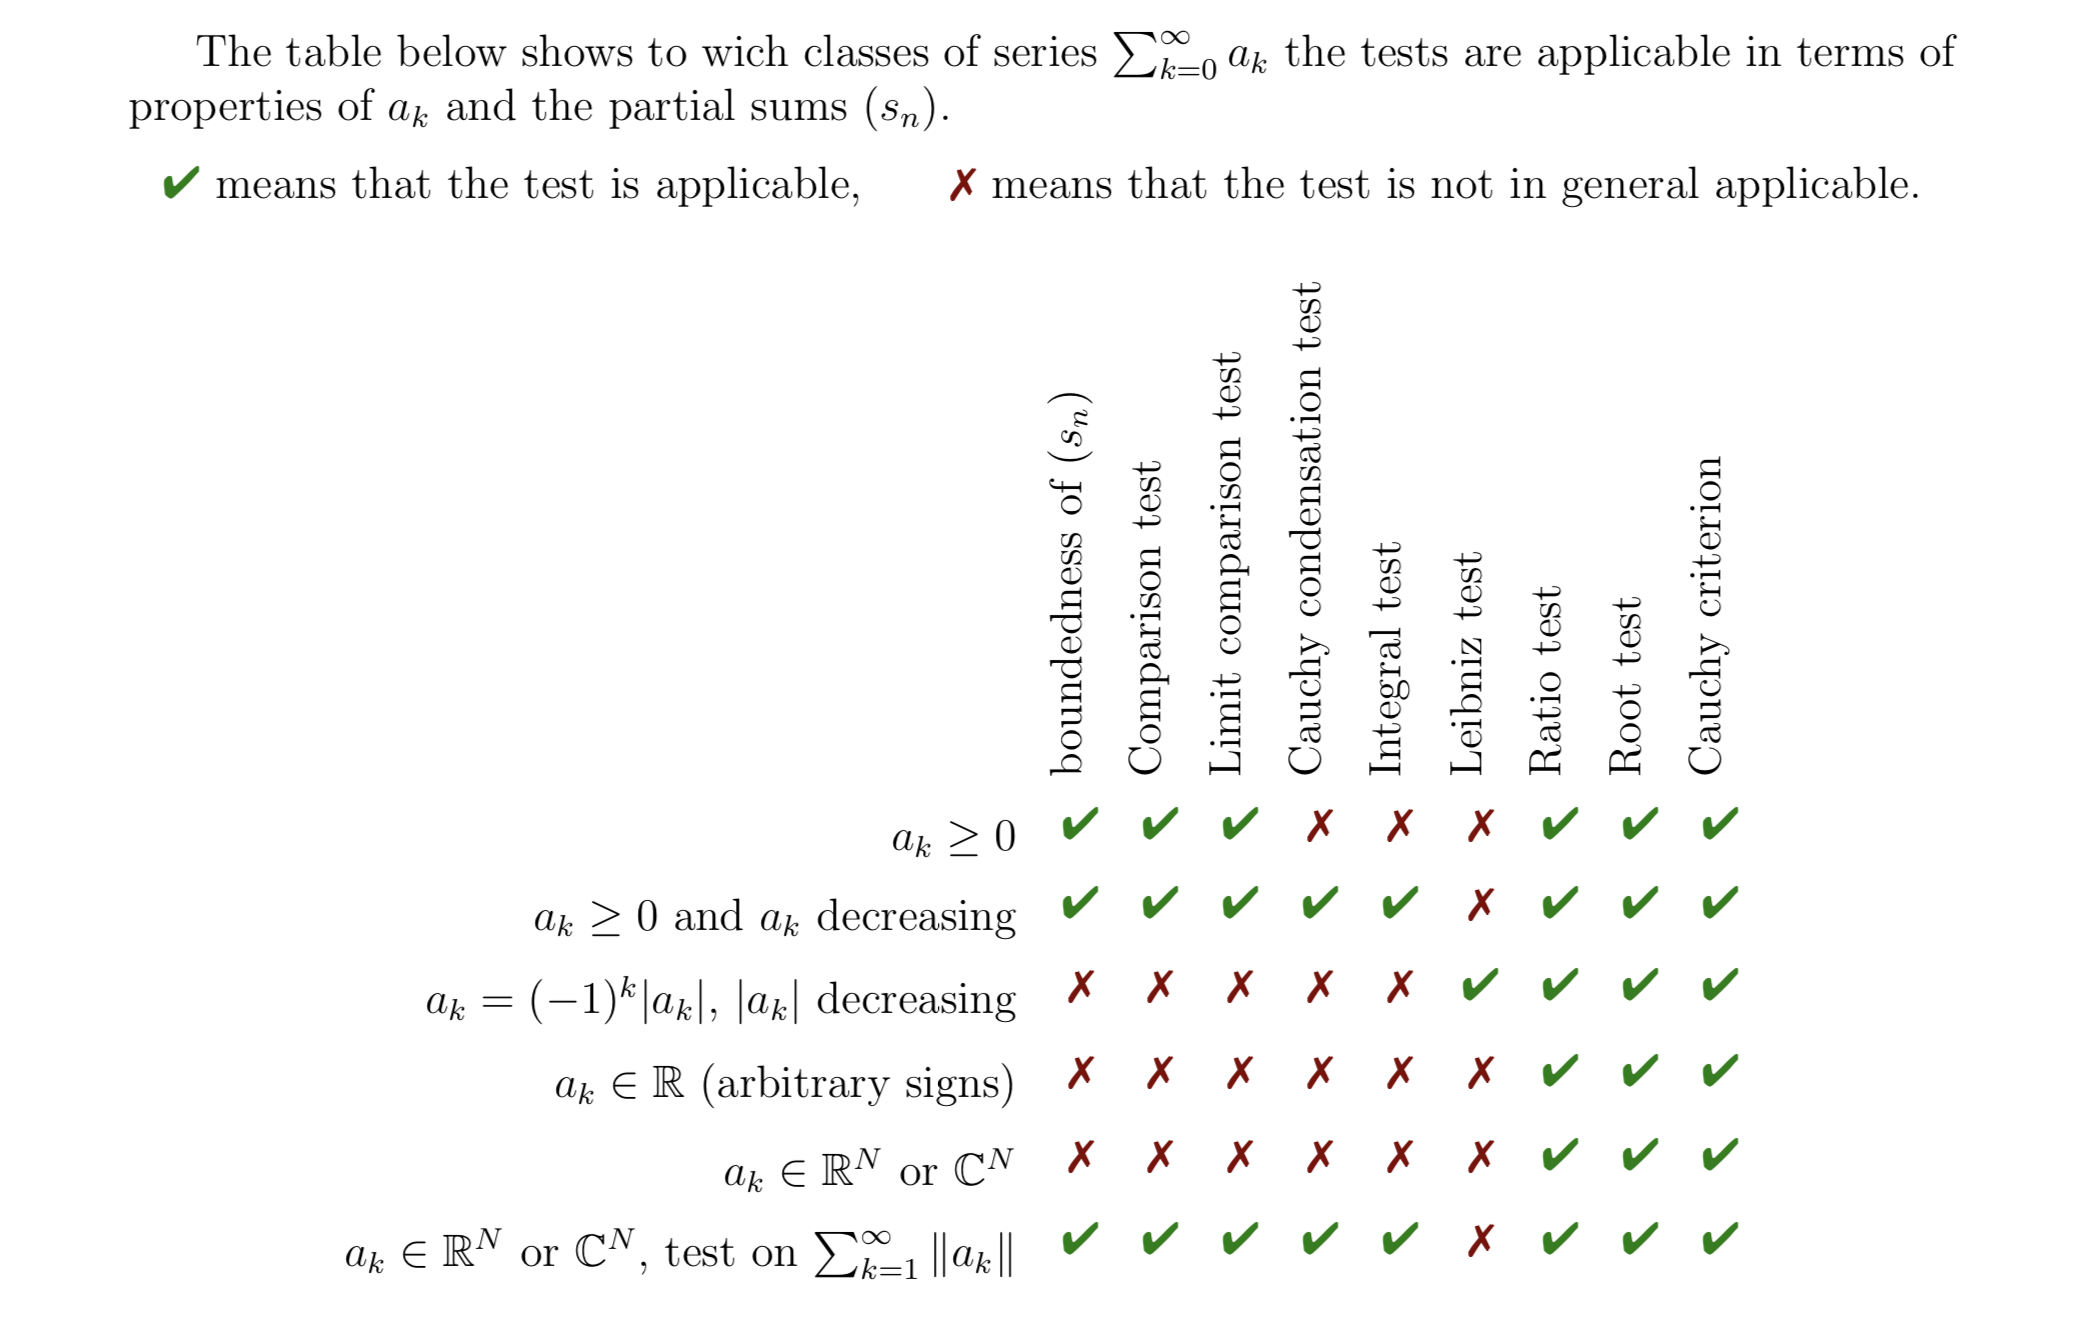
\includegraphics[width=18cm, height=12cm]{Assets/Series_tests.png}
\end{center}


\lecture{15}{Power Series and their Convergence Properties}
\section{Power Series and their Convergence Properties}
\subsection{Power Series and their Convergence Properties}
\begin{definition}(Power Series). Let $\{a_k\}_{k \geq 0}$ be a sequence in $\mathbb{K}^N$ and $x \in K$. Then the series
$$
\sum_{k=0}^{\infty}a_kx^k
$$
is called a $\textbf{power series}$ in $\mathbb{K}^N$. This is also known as the power series centered at 0. Furthermore, we can also look at the power series 
$$
\sum_{k=0}^{\infty}a_k(x - x_0)^k
$$
centered at $x_0 \in \mathbb{K}$.
\end{definition}

Here, we have a scalar x, which we raise to the power and multiply it by sequence. Power series has really nice convergence properties.

A power series will converge for certain values of x. There is an interval $(-\rho, \rho)$, where if $x \in (-\rho, \rho)$, then the power series converges. $\rho$ is known as the radius of convergence and if $\rho$ is within this interval, then the power series always converges absolutely, which then implies it also converges and hence it is unconditionally Convergent.

\begin{theorem}(Cauchy-Hadamard Theorem). Every power series $\sum_{k=0}^{\infty}a_kx^k $ in $\mathbb{K}^N$ either converges for all $x \in \mathbb{C}$ or there exists a $\rho \in [0,\infty)$ such that the series 
\begin{enumerate}
    \item converges absolutely for all $x \in \mathbb{C} $ if $\; |x| < \rho$;
    \item diverges for all $x \in \mathbb{C}$ if $\;|x| > \rho$;
    \item converges absolutely for every $x \in \mathbb{C}$ (where we set $\rho \coloneqq \infty$);
    \item diverges for every $x \in \mathbb{C} /\{0\}$ (where we set $\rho$ = 0).
\end{enumerate}

Additionally, for $|x| = \rho$, anything can happen and hence the behaviour is not defined and depends on the series.

Morever, we define
$$
\rho = \frac{1}{\Lim{n \rightarrow \infty}sup\sqrt[n]{||a_n||}}
$$
where we set $1/\infty \coloneqq 0$ and $1/0 \coloneqq \infty$.
\end{theorem}

\begin{definition}(Radius of Convergence). The number $\rho \in [0,\infty)$ defined above is known as the radius of convergence of the power series $\sum_{k=0}^{\infty}a_kx^k$. The radius of convergence can be derived in multiple ways.

(Root Test).
$$
\rho = \frac{1}{\Lim{n \rightarrow \infty}sup\sqrt[n]{||a_n||}}
$$

(Ratio Test).
$$
\rho = \Lim{n \rightarrow \infty}\frac{||a_n||}{||a_{n+1}||}
$$

\end{definition}

\begin{remark} Note that when using the root test, the n-th root must match the power of z. That is, if we had $z^{2n}$, then we need to use $\sqrt[2n]{||a_n||}$
\end{remark}


\begin{remark} We have that a power series converges uniformly and absolutely in any region that $\textbf{lies entirely}$ inside its circle of convergence. So we can express convergence in 2 ways. We can that it converges uniformly on any ball $b(0,r)$ with $r < \rho$ OR it converges locally uniformly on $b(0,\rho)$.
\end{remark}


\begin{remark} Using ratio test for $\rho$, if it is 1 or $\infty$. However, for root test, if we get 1/0, we say it is $\infty$, so it converges everywhere and if we get $1 / \infty = 0$, it diverges everywhere. 
\end{remark}



\lecture{16}{Double Series}
\section{Double Series}
\subsection{Double Series}
\begin{definition}(Double Series). A double series is defined to be
$$
\sum_{j,k=0}^{\infty}x_{jk}.
$$
This can be thought of as an infinite 2 dimensional array.
\end{definition}

There are many ways to add them up. This matters as the limit may depend on the order of summation.
\begin{enumerate}
  \item Sum by rows $$\sum_{j=0}^{\infty}\big(\sum_{k=0}^{\infty}x_{jk}\big)$$
  \item Sum by columns $$\sum_{k=0}^{\infty}\big(\sum_{j=0}^{\infty}x_{jk}\big)$$
  \item Sum by a bjiection $\sigma: \mathbb{N} \rightarrow \mathbb{N} \times \mathbb{N}$ $$\sum_{i=0}^{\infty}x_{\sigma(i)}$$.
\end{enumerate}

\begin{theorem}(Absolute Convergence for Double Series). Suppose that $x_{jk} \in \mathbb{K}^N$ are such that
$$
M \coloneqq \sup_{m,n \in \mathbb{N}}\sum_{j=0}^m\big(\sum_{k=0}^{n}||x_{jk}||\big) < \infty.
$$
Then the series of summing over rows/columns/bijection converges absolutely and 
$$
\sum_{j=0}^{\infty}\big(\sum_{k=0}^{\infty}x_{jk}\big) = \sum_{k=0}^{\infty}\big(\sum_{j=0}^{\infty}x_{jk}\big) = \sum_{i=0}^{\infty}x_{\sigma(i)}
$$
for every bijection $\sigma: \mathbb{N} \rightarrow \mathbb{N} \times \mathbb{N}$.
\end{theorem}

\begin{proof}(Sketch). To prove the absolute convergence of the three series, we have that $\sum_{j=0}^m||x_{j,k}|| \leq M$ for every $m,k \in \mathbb{N}$. The series converges as the sequence of partial sums here is bounded and hence the series converges absolutely. We repeat this argument for other 2 series. 

To prove equality of the limits, we can look at partial sums and use the definition of absolute convergence. We then take limits.
\end{proof}

A series that is absolutely convergent is unconditionally convergent, that is, the terms can be rearranged without changing the limit. Recall that the converse does not hold since taking the norm of vectors can stop things from cancelling out with each other and hence we get a different value. We can apply our double series absolute convergence to our original series.

\begin{corollary}(Absolutely Convergent Series are Unconditionally Convergent). Suppose that $\sum_{k=0}^{\infty}a_k$ is an absolutely convergent series in $\mathbb{K}^N$ and that $\sigma: \mathbb{N} \rightarrow \mathbb{N}$ is a bijection. Then $\sum_{k=0}^{\infty}a_{\sigma(k)}$ is absolutely convergent and
$$
\sum_{k=0}^{\infty}a_k = \sum_{j=0}^{\infty}a_{\sigma(j)}.
$$
\end{corollary}

Any permutation of a absolutely convergent series still converges to the same limit.

We now look at another application by looking at the product of two convergent series $a_j$ and $b_k$. We can have that
$$
ab = \sum_{j=0}^{\infty}\big(\sum_{k=0}^{\infty}a_jb_k\big) = \sum_{k=0}^{\infty}\big(\sum_{j=0}^{\infty}a_jb_k\big).
$$
Here, we have that the first row of our new array is $a_0b_k$ for $k \in \mathbb{N}$. Additionally, we have the first column of our array is $a_jb_0$ for $j \in \mathbb{N}$. We can also construct products by multiplying via diagonals instead. 

\lecture{17}{Cauchy Products}
\section{Cauchy Products}
\subsection{Cauchy Products}

\begin{definition}(Cauchy Products).
For 2 series $a_j$ and $b_k$, we can express the two series as
$$
c_n \coloneqq \sum_{k=0}^{n}a_kb_{n-k}.
$$
where $c_n$ is known as the $\textbf{Cauchy product}$ of the series a and b. We collect the new series by its diagonal.
\end{definition} 

\begin{theorem}(Convergence of Cauchy Products). Suppose that $a = \sum_{j=0}^{\infty}$ and $b = \sum_{k=0}^{\infty}b_k$ are absolutely convergent series in $\mathbb{K}$. Then their Cauchy product converges absolutely and
$$
\big(\sum_{j=0}^{\infty}a_j\big)\big(\sum_{k=0}^{\infty}b_k\big) = \sum_{n=0}^{\infty}\big(\sum_{k=0}^na_kb_{n-k}\big).
$$
\end{theorem}

\begin{proof}
The conditions of the double series theorem is satisfied and hence this is also satisfied. In particular,
$$
\sum_{j=0}^{\infty}(\sum_{k=0}^{n}|a_jb_k|) = \sum_{j=0}^{m}(|a_j|)(\sum_{k=0}^{n}|b_k|) \leq \sum_{j=0}^{\infty}(|a_j|)(\sum_{k=0}^{\infty}|b_k|) \coloneqq M < \infty.
$$

\end{proof}

\begin{example}Recall that for the exponential function, we have
$$
exp(x) = \sum_{k=0}^{\infty}\frac{x^k}{k!}
$$
and this converges absolutely for all $x \in \mathbb{C}$. We compute the Cauchy product of exp(x) and exp(y).

We use the Binomial theorem after introduction $n!/n!$.
$$
c_n = \sum_{k=0}^n\frac{x^k}{k!}\frac{y^{n-k}}{(n-k)!} = \frac{1}{n!}\sum_{k=0}^n\frac{n!}{k!(n - k)!}x^ky^{n-k} = \frac{1}{n!}\sum_{k=0}^n{n \choose k}x^ky^{n-k} = \frac{(x+y)^n}{n!}
$$
for all $n \in \mathbb{N}$. Hence,

$$
exp(x)exp(y) = \sum_{n=0}^{\infty}\frac{(x+y)^n}{n!} = exp(x+y).
$$
\end{example}

\lecture{18}{Closed and Open Sets}
\section{Closed and Open Sets}
\subsection{Closed and Open Sets}

We now look at Topology of sets. First, we describe functions using open and closed subsets of $\mathbb{K}^N$. We use these sets to also help us describe limits and continuity. To define open sets, we use $\textbf{open balls}$.

\begin{definition}(Open Ball). Let $x \in \mathbb{K}^N$ and pick a $r > 0$. We call
$$
B(x,r) \coloneqq \{y \in \mathbb{K}^N: ||y-x|| < r\}
$$
the open ball about x with radius r.
\end{definition}

From this, we can define open sets.
\begin{definition}(Open Sets). A set $U \subseteq \mathbb{K}^N$ is called open if either $U = \emptyset$ or for every $x \in U$, there exists $r > 0$ such that
$$
B(x,r) \subseteq U.
$$
\end{definition}

In other words, for every element in the set, we can find a radius r in order to fit a ball around the element and still be contained within the set.

\begin{definition}(Closed Sets). A set is closed if its complement is open.
\end{definition}

\begin{lemma}An open ball B(x,r) is an open set.
\end{lemma}
\begin{proof}
We show that for every $z \in B(x,r)$, there exists $\epsilon>0$ such that $B(z,\epsilon) \subseteq B(x,r)$. Set distance $\epsilon$ to be the size of ball subtract the distance from x to z. First fix an element $z \in B(x,r)$. Then set $\epsilon \coloneqq r - ||x-z||$. If $y \in B(z,\epsilon)$, then $||y-z|| < \epsilon$. Hence, we have that by triangle inequality
$$
||y-x|| = ||y-z+z-x|| \leq ||y-z|| + ||z-x||
$$
$$
< \epsilon + ||z-x|| = r - ||x-z|| + ||z-x|| = r.
$$
Therefore, $||y-x|| < r$, that is, $y \in B(x,r)$. Hence, $B(z,\epsilon) \subseteq B(x,r)$ as required which shows that $B(x,r)$ is open.
\end{proof}

We now derive properties of open sets in $\mathbb{K}^N$.

\begin{proposition}(Basic properties of open sets). Open sets have the following properties:
\begin{enumerate}[(i)]
  \item $\emptyset$ and $\mathbb{K}^N$ are open sets;
  \item The union of an arbitrary collection of open sets is open;
  \item The intersection of $\textbf{finitely}$ many open sets is open.
\end{enumerate}
\end{proposition}

\begin{proof}
(i) This is true by definition. 

(ii) Choose an $x \in \bigcup_{i \in I}U_i$. This means that $x \in U_j$ for some $j \in I$. Then that means there exists $r > 0$ such that $B(x,r) \subset U_j$ which is a subset of $\bigcup_{i \in I}U_i$. Hence, this works for every choice x and therefore $\bigcup_{i \in I}U_i$ is open.

(iii) Let $x \in \bigcap_{i=1}^nU_i$. This means that $x \in U_i$ for every i=1,2,...,n. Since $U_i$ is open, there exists $r_i > 0$ such that $B(x,r_i) \subseteq U_i$. We let 
$$
r \coloneqq min\{r_1,...,r_n\}.
$$
Note that this is the reason we require a finite number of open sets as a list of infinite numbers is not guaranteed to have a minimum. Hence, then that means $B(x,r) \subset \bigcap_{i=1}^nU_i$ and as this works for every $x \in \bigcap_{i=1}^nU_i$, this means that $\bigcap_{i=1}^nU_i$ is open.
\end{proof}

\begin{remark} An example of the intersection of infinitely many open sets not being open can be
$$
\bigcap_{i=0}^{\infty}(0, 1 + \frac{1}{i}) = (0,1]
$$
which is not open nor closed.
\end{remark}


\begin{proposition}(Basic properties of closed sets). Closed sets have the following properties:
\begin{enumerate}[(i)]
  \item $\emptyset$ and $\mathbb{K}^N$ are closed sets;
  \item The intersection of an arbitrary collection of closed sets is closed;
  \item The union of an arbitrary collection of finitely many closed sets is closed.
\end{enumerate}
\end{proposition}

\begin{proof}(i) This holds from the definition of closed sets as the complement $\mathbb{K}^N$ and $\emptyset$ is open.

(ii) Let $(A_i)_{i \in I}$ be an arbitrary collection of closed subsets of $\mathbb{K}^N$. Let $U_i \coloneqq A_i^c$ be open by the definition of closed sets for all $i \in I$. Hence, $\cup_{i \in I}U_i$ is open from earlier statement. Using De Morgan's Law
$$
\big(\bigcap_{i \in I}A_i\big)^c = \bigcup_{i \in I}A_i^c = \bigcup_{i \in I}U_i
$$
is open. Therefore, by definition of closed sets, $\cup_{i=1}^nA_i$ is closed.

(iii) Let $A_i$ for i=1,...,n be closed subsets of $\mathbb{K}^N$. Then $U_i \coloneqq A_i^c$ is open by definition of closed sets. Then, $\cap_{i=1}^nU_i$ is open. Be De Morgan's Law, 
$$
\big(\bigcup_{i \in I}A_i\big)^c = \bigcap_{i \in I}A_i^c = \bigcap_{i \in I}U_i
$$
is open. Hence, $\bigcup_{i=1}^nA_i$ is closed by definition of a closed set.
\end{proof}

\begin{remark} An example of the union of infinitely many closed sets not being closed can be
$$
\bigcup_{i=0}^{\infty}[\frac{1}{i}, 1] = (0,1]
$$
which is not closed nor open.
\end{remark}

Note that the reason we need a finite union of closed sets, is because we look at the complement, which is the intersection of open sets, which requires to be finite in order for earlier argument to apply.

Note that sets can be both open and closed. Also, sets that are not closed does not mean they are open and vice versa. To check whether a set is open, make sure you can always find a r for each point in the set such that the ball around that set is contained within the set.


\begin{proposition} A set A that is closed and bounded from above(below) admits a maximum(minimum).
\end{proposition}

\begin{proof} Since the set A is bounded from above, by the least upper bound axiom, it has a supremum $\mathcal{M}$. Then, by definition of a supremum, for every $\epsilon > 0$, there exists $a \in A$ such that
$$
\mathcal{M} - \epsilon < a < \mathcal{M}.
$$

SO then, $B(\mathcal{M}, \epsilon) \cap A \neq \emptyset$ for all $\epsilon > 0$. So then $\mathcal{M}$ is in the closure of A. However, the closure of a closed set is the set itself. Hence, $\mathcal{M}$ is in A and is therefore the maximum.
\end{proof}


Sometimes, it is more convenient to replace the base set $\mathbb{K}^N$ by a subset $D \subseteq \mathbb{K}^N$. This may be because we want the "universe" of points we want to analyse be from D rather than $\mathbb{K}^N$.

\begin{definition}(Relatively Open Sets). Let $D \subseteq \mathbb{K}^N$, which is our new domain. The set $U \subseteq D$ is called relatively open in D if $U \neq \emptyset$ or for every $x \in U$, there exists $r > 0$ such that $B(x,r) \cap D \subseteq U$.
\end{definition}

\begin{remark}Just for intution on why we need $B(x,r) \cap D$, is because for every point x, we look at all the points in $\mathbb{K^N}$ that is within the ball of x. However, the point of relatively open sets is that D is now "our universe" rather than $\mathbb{K}^N$ and hence there isn't any purpose to looking at points outside of our universe, which is D. Hence, the reason we put a restriction at only looking at points in the ball that are also in our universe.
\end{remark}

\begin{definition}(Relatively Closed Sets). $A \subseteq D$ is called relatively closed in D if the complement of $A^c \cap D$ is relatively open in D.
\end{definition}

Here, we say U is open in D or A is closed in D. If $D = \mathbb{K}^N$, then open/closed is equivalent to relatively open/closed.

\begin{proposition}(Basic properties of relatively open sets). Let $D \subseteq \mathbb{K}^N$. Then, 
\begin{enumerate}[(i)]
  \item $\emptyset$ and D are open in D;
  \item Arbitrary unions of relatively open sets are open in D;
  \item Finite intersection of relatively open sets are open in D.
\end{enumerate}
\end{proposition}

These properties can be used to prove many properties of continuous functions. Furthermore, any collection of subsets of D with the above properties holding for D, is known as a $\textbf{topology}$.

\begin{definition}(Diameter of a set). Let $K_n \subset \mathbb{R}^N$ be a closed and non-empty set. The diameter of the set is 
$$
diam(K_n) \coloneqq \sup_{x,y \in K_n}||x - y|| \rightarrow 0.
$$
\end{definition}

\begin{proposition}(Cantor's Intersection Theorem). Let $K_n$ be a decreasing nested sequence of non-empty, closed and bounded sets of $\mathbb{R}$. The intersection is non-empty, that is 
$$
\bigcap_{n \in \mathbb{N}}K_n \neq \emptyset.
$$
\end{proposition}

\begin{proof}(Sketch). Show that $\{x_n\}$ is a Cauchy sequence. From that, show that the limit of the sequence is in every set $K_n$ and hence it is in the intersection.
\end{proof}

\begin{remark} Note that the intersection of open sets will be an empty set.
\end{remark}


\lecture{19}{Closures and their sequential characeterisation}
\section{Closures and their sequential characeterisation}
\subsection{Closures}

We first look at the standard definitions.

\begin{definition}(Interior Point). A point $x \in A$ is called an interior point of A if there exists $r > 0$ such that $B(x,r) \subseteq A$.
\end{definition}

\begin{definition}(Interior). The interior of the set A, is the set of all interior points of A.
$$
int(A) = \{x \in A: \text{ x is an interior point of A}\}.
$$
\end{definition}

\begin{definition}(Closure). The closure of the set A is the set of all points that are "close" to A. 
$$
\bar{A} = \{x \in \mathbb{K}^N: B(x,r) \cap A \neq \emptyset \textbf{ for all r} > 0\}
$$
\end{definition}

Notice that the closure requires for all radius r.

\begin{definition}(Boundary). The boundary of the set A are all the points in the closure of A that are $\textbf{not}$ in the interior of A.
$$
\partial A = \bar{A} - int(A).
$$
\end{definition}

However, these definitions can make building up other properties more cumbersome, hence we introduce more generalised definitions.

\begin{definition}(Interior of a set). Let $A \subseteq \mathbb{K}^N$. The interior of A, denoted by int(A), is the $\textbf{largest open set}$ in $\mathbb{K}^N$ that is $\textbf{included}$ in A. By definition, int(A) is open and $int(A) \subseteq A$. More precisely,
$$
int(A) = \bigcup\{U \subseteq \mathbb{K}^{N}: \text{ U is open and }U \subseteq A\}
$$
\end{definition}

Hence, if $int(A) = A \leftrightarrow A$ is open. 

We note that for something to be in the interior, we need to be able to find a radius such that the open ball around that point is also in the set A.

\begin{definition}(Closure of a set). The closure of a set A, denoted by $\bar{A}$ is defined as the $\textbf{smallest closed set}$ in $\mathbb{K}^N$ that $\textbf{contains}$ A. More precisely,
$$
\bar{A} = \bigcap\{F \subseteq \mathbb{K}^N: \text{ F is closed and } A \subseteq F\}.
$$
\end{definition}

Hence, if $\bar{A} = A \leftrightarrow A$ is closed.

\begin{proposition}Let $A \subseteq \mathbb{K}^N$. Then the following assertions are true.

\begin{enumerate}[(i)]
  \item The set int(A) is open. Moreover, A is open if and only if int(A) = A.
  \item The set $\bar{A}$ is closed. Moreover, A is closed if and only if $\bar{A} = A$.
\end{enumerate}
\end{proposition}

\begin{claim}
The complement of the closure of A is the interior of the complement of A. 
$$
(\bar{A})^c = Int(A^c).
$$
\end{claim}

\begin{proof}
We have that
$$
\bar{A} = \cap\{F \subseteq \mathbb{K}^N: \text{F is closed, } A \subseteq F\}
$$
$$
\big(\bar{A}\big)^c = \cup\{F^c \subseteq \mathbb{K}^N: F^c\text{ is closed, } F^c \subseteq A^c\}
$$
$$
= \cup\{U \subseteq \mathbb{K}^N: \text{U is open, } U \subseteq A^c\}
$$
$$
= int(A^c).
$$
where we have that $U = F^c$ and the last equality arising by definition.
\end{proof}

\subsection{Sequential characeterisation of closure}
We now make a connection between the closure of a set A and sequences in A. We want to look at the fact that all accumulation points of sequences in A lie in the closure $\bar{A}$. Furthermore, we can also show that every point in the closure $\bar{A}$ is the limit of a sequence in A. Hence, we can actually characterise the closure $\bar{A}$ as the set of points which are accessible by a sequence of points in A.
\begin{proposition}(Sequential Characterisation of closure). Let $A \subseteq \mathbb{K}^N$. Then we have 

(i) If $\{x_n\}$ is a sequence in A, which converges to $x \in \mathbb{K}^N$, then $x \in \bar{A}$;

(ii) If $x \in \bar{A}$, then there exists a sequence $\{x_n\}$ in A converging to x.
\end{proposition}

\begin{proof}
(i) First recall that the closure is $\bar{A} = \{x \in \mathbb{K}^N: \forall \; r > 0, B(x,r) \cap A \neq \emptyset \}$. As $x_n \rightarrow x$ as $n \rightarrow \infty$, combined with the fact that $x_n \in A$ for all $n \geq 0$, we have that for all $\epsilon > 0$, there exists $n_{\epsilon} \in \mathbb{N}$ such that $||x_n - x|| < \epsilon$ for all $n \geq n_{\epsilon}$. We can re-express this as $x_n \in B(x,\epsilon)$ for all $n \geq n_{\epsilon}$. We let $\epsilon = r$ and hence we have that $x_n \in B(x,r) \cap A$ for all $n \geq n_{\epsilon}$. Therefore, we get the claim that $x \in \bar{A}$ as $B(x,\epsilon) \cap A \neq \emptyset$.

(ii) If $x \in \bar{A}$, then by definition of $\bar{A}$, the sets $B(x,r) \cap A \neq \emptyset$ for all $r > 0$. In particular, for every $n \in \mathbb{N}$, we can choose $x_n \in B(x, 1/n) \cap A \neq \emptyset$. Hence, there exists $x_n \in A$ and $||x_n - x|| \rightarrow 0$, that is, $x_n \rightarrow x$. Hence, we have found the sequence needed.

\end{proof}

We can now use this proposition on closed sets.
\begin{proposition}(Sequential characterisation of closed sets). For a set $A \subset \mathbb{K}^N$, then we have that A is closed if and only if every convergent sequence in A has its limit in $A \subseteq \mathbb{K}^N$.
\end{proposition}

\begin{proof}
We use that the closure of a closed set is itself.

$\rightarrow$

If A is closed, then $A = \bar{A}$. Then, let $\{x_n\}$ be a sequence in A which converges to x. From the sequential characterisation of closures, the limit x is in $\bar{A}$. However, as the closure of A is itself, then that means that $x \in A$.

$\leftarrow$

First, we note that $A \subseteq \bar{A}$ by definition of $\bar{A}$. Then, we assume that every sequence in A has its limit in A. We need to show that $\bar{A} \subseteq A$ to show $A = \bar{A}$ and hence A is closed. We pick an arbitrary $x \in \bar{A}$ and from the sequential characteristic of closures, then there exists a sequence in A that converges to x. However, we already assumed that the limit $x \in A$. Therefore, $\bar{A} \subseteq A$, which then shows that $\bar{A} = A$ and can only be true if A is closed.
\end{proof}

This characterisation makes sense, as we know that the limit point of a sequence is in the closure of the set and since a closed set's closure is itself, then the limit point must also be in the closed set.

\lecture{20}{Limits and Continuity of Functions}
\section{Limits for Functions}
\section{Limits and Continuity}
\subsection{Limits for Functions}

\begin{definition}(Limits for functions). Let $f: D \rightarrow \mathbb{K}^N$ be a function with domain $D \subseteq \mathbb{K}^d$ and $x_0 \in \bar{D}$ Let $b \in \mathbb{K}^N$.

(i) We say that f(x) converges to b as x approaches $x_0$ if for every $\epsilon > 0$, there exists $\delta(\epsilon) > 0$ such that
$$
||f(x) - b|| < \epsilon
$$
for all $x \in D/\{x_0\}$ with $0 < ||x - x_0|| < \delta(\epsilon)$. We write
$$
f(x) \rightarrow b \;as\;x \rightarrow x_0 \;\;\; or \;\;\; b = \Lim{x \rightarrow x_0}f(x).
$$

(ii) Suppose that $D \subseteq \mathbb{R}$ is not bounded from above. Then $b = \Lim{x \rightarrow \infty}f(x)$ if for every $\epsilon > 0$, there exists $\delta(\epsilon) > 0$ such that
$$
||f(x) - b|| < \epsilon
$$
for all $x \in D$ with $x > \delta(\epsilon)$.
\end{definition}

Here, note that we have a sequence in the domain approaching $x_0$ with is in the closure $\bar{D}$, not necessarily in D. Additionally, (ii) looks at finding the rank $\delta$ for which $f(x)$ is within an $\epsilon$ neighbourhood of b.


We can formulate the definition of a limit in many ways.
\begin{proposition}The following assertions are equivalent.

(i) $\Lim{x \rightarrow x_0}f(x) = b$;

(ii) For every $\epsilon > 0$, there exists $\delta(\epsilon) > 0$ such that $f(x) \in B(b,\epsilon)$ for all $x \in B(x_0, \delta(\epsilon)) \cap D/\{x_0\}$ with $x \neq x_0$;

(iii) $\Lim{n \rightarrow \infty}f(x_n) = b$ $\textbf{for every sequence}$ $\{x_n\}$ in $D/\{x_0\}$ with $x_n \rightarrow x_0$ and $x_n \neq x_0$ for all $n \in \mathbb{N}$.
\end{proposition}

\begin{proof}
(i) $\rightarrow$ (ii) by the definition of the limit and the open ball.

(i) $\rightarrow$ (iii) Assume that $\Lim{x \rightarrow x_0}f(x) = b$. Then, by definition, we have that for all $\epsilon > 0$, there exists $\delta = \delta(\epsilon) > 0$ such that
$$
||f(x) - b|| < \epsilon
$$
for all $x \in D/\{x_0\}$ with $||x-x_0|| < \delta$. Let $\{x_n\}$ be a sequence in $D/\{x_0\}$ with $\Lim{n \rightarrow \infty}x_n = x_0$. Fix $\epsilon > 0$ to be arbitrary. Then there exists $n_{\delta} \geq n$ such tht 
$$
||x_n - x_0|| < \delta
$$
for all $n \geq n_{\delta}$. Hence, we have that $||f(x_n) - b|| < \epsilon$ for all $n \geq n_{\delta}$. This gives us that $\Lim{n \rightarrow \infty}f(x_n) = b$.

(iii) $\rightarrow$ (i). (Contradiction). Assume that $\Lim{x \rightarrow x_0}f(x) \neq b$. Then, there exists $\epsilon_{0} > 0$ such that for all $\delta > 0$, there exists $x_{\delta} \in D/\{x_0\}$ with $||x_{\delta} - x_0|| < \delta$ such that $||f(x_{\delta} - b)|| > \epsilon_0$. Let $\{\delta_n\}$ be a sequence of positive numbers converging to 0. (For example, $\delta_n = \frac{1}{n}$). Then, there exists $x_n \in D/\{x_0\}$ with $0 \leq ||x_n - x_0|| < \delta_n = \frac{1}{n}$ and $||f(x_n) - b|| \geq \epsilon_0$. By the squeeze law, $x_n \rightarrow x_0$ as $n \rightarrow \infty$. We get a contradiction as $\Lim{n \rightarrow \infty}f(x_n) = b$, but we assumed that the limit was not b.
\end{proof}

\begin{remark}
For (ii), we require x to be in the domain D and hence why we take the intersection with D. We are not interested in points outside of the domain, similar to the example with the relatively open sets.

The equivalence of (i) and (iii) allows us to apply results on limits of sequences to limits of functions.
\end{remark}

\subsection{Continuity of Functions}

\begin{definition}(Continuity). The function $f: D \rightarrow \mathbb{K}^N$ is said to be continuous at $x_0 \in D$ if $\Lim{x \rightarrow x_0}f(x) = f(x_0)$. Moreover, f is said to be continuous if it is continuous at every $x \in D$. We define the set
$$
C(D, \mathbb{K}^N) \coloneqq \{f: D \rightarrow \mathbb{K}^N: \text{f is continuous}\}
$$
and call it the space of continuous functions from D into $\mathbb{K}^N$.
\end{definition}

Note that we require $x \in D$, not just $x \in \bar{D}$ in order for $f(x_0)$ to be defined and make sense. However, if $\Lim{x \rightarrow x_0}f(x)$ exists for a $x_0 \not \in D$ but in $x \in \bar{D}$, we can extend the domain to be $D \cup \{x_0\}$ and hence the new function is continuous after we define $f(x_0) \coloneqq b$. 

\begin{proposition}(Characterisation of continuity of functions). If for all U open in $\mathbb{K}^N$, then $f^{-1}(U) = \{x \in D: f(x) \in U\}$ is relatively open in D, then f is continuous.

If for all A closed in $\mathbb{K}^N$, then $f^{-1}(A)$ is relatively closed in D.
\end{proposition}
The set $C(D, \mathbb{K}^N)$ is a vector space over $\mathbb{K}$ if we define addition and mutliplication by scalars $\textbf{pointwise}$. By limit laws, f+g and $\alpha f$ are continuous if $f$ and $g$ are continuous with $\alpha \in \mathbb{K}$. Note that this vector is only finite dimensional.

\subsection{Properties of Continuous Functions}

Here, we will prove some properties of continuous functions on closed and bounded sets of $\mathbb{K}^N$. We will need to use the Bolzano-Weierstrass Theorem that asserts that every bounded sequence in $\mathbb{K}^N$ has a convergent subsequence.

\begin{definition}(Bounded set). A set $A \subseteq \mathbb{K}^N$ is called bounded if there exists $R \geq 0$ such that $||x|| \leq R$ for all $x \in A$.
\end{definition}

Geometrically, you can think of it as the set A being able to be fit into a large enough ball. We can use the following result that helps us to determine whether a set is bounded based on its sequences.

\begin{proposition}The set $A \subseteq \mathbb{K}^N$ is bounded if and only if every sequence in A has a convergent subsequence.
\end{proposition}

\begin{proof} 

$\rightarrow$

Suppose that A is bounded and has a sequence $(x_n)$ in A. This sequence will also be bounded. By the Bolzano-Weierstrass theorem, this bounded sequence will have a convergent subsequence.

$\leftarrow$(Contrapositive).

Suppose that A is not bounded. Then, for every $n \in \mathbb{N}$, there exists $x_n \in A$ such that $||x_n|| \geq n$. Hence, we have found a sequence $(x_n)$ in A where every subsequence is unbounded and therefore divergent. Hence it has no divergent subsequence. By the contrapositive, this means that a sequence with a convergent subsequence implies that the set is bounded.
\end{proof}

We can further characterise $\textbf{compact}$ sets, which in this case are $\textbf{closed and bounded}$ sets.

\begin{definition}(Sequentially Compact Sets). A set A, where every sequence in A has a convergent subsequence with limit in A.
\end{definition}

\begin{corollary} For a set $A \subseteq \mathbb{K}^N$, we have that a set A is closed and bounded if and only if A is sequentially compact.
\end{corollary}

\bigskip
Continuous functions carries compact sets to compact sets.

\begin{theorem}Let $f \in C(D, \mathbb{K}^N)$ with $D \subseteq \mathbb{K}^d$. If $A \subseteq D$ is closed and bounded, then its image $$f(A) = \{y \in \mathbb{K}^N: \text{there exists } x \in A \;\;s.t. \; f(x) = y\}$$ is also closed and bounded.
\end{theorem}

\begin{proof}
To prove that $f(A)$ is a compact subset of $\mathbb{K}^N$, it is enough to show that any sequence $\{y_n\}$ in f(A) contains a convergent subsequence with the limit in f(A).

Let A be closed and bounded. Let $\{y_n\}$ be a sequence in f(A). Then for every $n \in \mathbb{N}$, there exists $x_n \in A$ with $f(x_n) = y_n$. Since A is bounded, $\{x_n\}$ has a convergent subsequence $\{x_{n_k}\}$ with $x_{n_k} \rightarrow x$ as $k \rightarrow \infty$. Since A is closed, $x \in A$. 

By continuity of f, 
$$
y_{n_k} = f(x_{n_k}) \rightarrow f(x) \in f(A) \;\;\; as \;k \rightarrow \infty.
$$

Hence, $\{y_n\}$ has a convergent subsequence with limit in f(A). Hence, f(A) is sequentially compact. This shows that f(A) is closed and bounded.
\end{proof}

Using the characterisation of continuity involving closed sets, we can prove the following fact on inverse functions.

\begin{proposition}(Continuity of inverse functions). Let $D \subseteq \mathbb{K}^d$ be compact (closed and bounded) and $f \in C(D, \mathbb{K}^N)$ injective. Then the inverse function $f^{-1}: f(D) \rightarrow \mathbb{K}^d$ is continuous.
\end{proposition}

\begin{proof} Suppose $A \subseteq \mathbb{K}^d$ is closed. Then we know that the image of $(f^{-1})^{-1}[A] = f(A \cap D)$ is closed and bounded since $A \cap D$ is closed and bounded. Hence, the pre-image of every closed subset $A \subseteq \mathbb{K}^d$ under $f^{-1}$ is closed. Hence, the inverse is continuous.
\end{proof}

We also derive another property of functions on closed and bounded sets.

\begin{theorem}(Extreme Value Theorem). Any real-value function that is continuous on a compact (closed and bounded) subset of $\mathbb{K}^d$ attains a maximum and minimum. In other words, if $f \in C(D,\mathbb{R})$, then there exists a,b $\in$ D such that 
$$
m \coloneqq f(a) \leq f(x) \leq f(b) \coloneqq M
$$
for all $x \in D$. Here, m is the $\textbf{minimum}$ and M is the $\textbf{maximum}$. So the domain D is closed and bounded.
\end{theorem}

\begin{proof}
Since D is a compact subset of $\mathbb{K}^d$ and $f: D \rightarrow \mathbb{R}$ is continuous, we know that f(D) is also compact from the previous theorem. Hence, f(D) is a closed and bounded subset of $\mathbb{R}$. By the completeness of $\mathbb{R}$, we infer that a sup f(D) and inf f(D) exists in $\mathbb{R}$ (as we have a bounded set). f(D) is closed so that f(D) contains all its accumulation points. As the infimum and supremum is also an accumulation point, this implies that 
$$
\sup f(D) \in f(D) \;\;\; and \;\;\; \inf f(D) \in f(D).
$$
As the supremum and infimum is within the set, this means that we have a $\textbf{maximum}$ and $\textbf{minimum}$ for f(D).
\end{proof}

Continuous functions can be characterised by open or closed sets. 
\begin{proposition}Let $D \subseteq \mathbb{R}^d$ and $f: D \rightarrow \mathbb{R}^N$ be a function. Given the set $U \subseteq \mathbb{R}^N$, we define the $\textbf{inverse image}$ or the $\textbf{pre-image}$ to be the set
$$
f^{-1}[U] \coloneqq \{x \in D: f(x) \in U\}.
$$

Furthermore, the following statements are equivalent.
\begin{enumerate}[(i)]
  \item $f: D \rightarrow \mathbb{R}^N$ is continuous;
  \item $f^{-1}[U]$ is open in D for every open set $U \subseteq \mathbb{R}^N$;
  \item $f^{-1}[A]$ is closed in D for every closed set $A \subseteq \mathbb{R}^N$.
\end{enumerate}
\end{proposition}

\begin{remark}Note that the image of an open or closed set does not need to be open or closed respectively!
\end{remark}

\begin{remark}If the set A is compact and f is continuous, then f(A) is compact. Resultantly, a continuous function on a compact set into $\mathbb{R}$ has a maximum and a minimum.
\end{remark}

\lecture{21}{Uniform Continuity and Convergence}
\section{Uniform Continuity}
\subsection{Uniform Continuity}

Another consequence of compactness of sets is the idea of uniform continuity. We can now look at stronger definitions of continuity. Usually for continuity, $\delta$ depends on $\epsilon$ and $x_0$. However, if the domain is compact, $\delta$ is now independent of the point $x_0 \in D$.

\begin{definition}(Uniform Continuous). Let $D \subseteq \mathbb{K}^d$ and $f: D \rightarrow \mathbb{K}^N$. We say that f is uniformly continuous on D if for all $\epsilon > 0$, there exists $\delta = \delta(\epsilon) > 0$ such that
$$
||f(x) - f(y) || < \epsilon
$$
for all x,y $\in D$ with $||x-y|| \;< \;\delta$.
\end{definition}

\begin{remark}
The difference between this and continuous function is that for a continuous function we had that for a function $f: D \rightarrow \mathbb{K}^N$, then it is continuous on D if it is continuous at each point in D, that is, for all $x \in D$ and for all $\epsilon > 0$, there exists $\delta = \delta(x,\epsilon) > 0$ such that 
$$
||f(x) - f(y) || < \epsilon
$$
for all x,y $\in D$ with $||x-y|| < \delta$.

In the case of a continuous function, the $\delta$ depends on both x and $\epsilon$, whilst for uniform continuous functions, it only depends on $\epsilon$.
\end{remark}
Therefore, we have the statement that
\begin{center}
$\textit{A uniform continuous function implies a continuous function.}$
\end{center}
Here, $\delta$ must be the same for all x for uniform continuity. The converse does not hold.

\begin{theorem}Any continuous function from a compact subset of $\mathbb{K}^d$ to $\mathbb{K}^N$ is uniformly continuous.
\end{theorem}

\begin{proof}
Let $f: D \rightarrow \mathbb{K}^N$ be continuous and $D \subseteq \mathbb{K}^d$ is a compact subset. Assume by contradiction, that f is not uniformly continuous. That is, there exists an $\epsilon_0 > 0$ such that for all $\delta > 0$, there exists $x_{\delta}, y_{\delta} \in D$ with
$$
||x_{\delta} - y_{\delta}|| < \delta
$$
for which
$$
||f(x_{\delta}) - f(y_{\delta})|| \geq \epsilon_0.
$$
Let $\{\delta_n\}_{n \geq 1}$ be a sequence of positive numbers converging to 0. (For example, $\delta_n = \frac{1}{n}$ for $n \geq 1$). Then, there exists $\{x_n\}$ and $\{y_n\}$ in D such that
$$
||x_n - y_n|| < \frac{1}{n} \;\;\; \forall n \geq 1
$$
$$
||f(x_n) - f(y_n)|| \geq \epsilon_0 \;\;\; \forall n \geq 1.
$$
Since D is compact, we have that D is sequentially compact. Then, there exists a subsequence $\{x_{n_k}\}$ converging to x in D. Using that
$$
0 < ||x_{n_k} - y_{n_k}|| < \frac{1}{n_k}
$$
for all $k \geq 1$ and $\Lim{k \rightarrow \infty}x_{n_k} = x$. We conclude that
$$
\Lim{k \rightarrow \infty}y_{n_k} = x.
$$
We arrive at a contradiction of
$$
0 \leq ||y_{n_k} - x|| \leq ||y_{n_k} - x_{n_k}|| + ||x_{n_k} - x||
$$
where the last 2 terms goes to 0 as $k \rightarrow \infty$. 

Recall that
$$
||f(x_n) - f(y_n)|| \geq \epsilon_0
$$
for all $n \geq 1$. Tus, taking $n_k$ instead of n, we get that
$$
||f(x_{n_k} - f(y_{n_k}))|| \geq \epsilon_0
$$
for all $k \geq 1$. 

Take $k \rightarrow \infty$ in the above inequality to obtain that
$$
||f(x) - f(x) || \geq \epsilon_0.
$$

We use the continuity of f, where by
$$
f(x_{n_k}) \rightarrow f(x) \;\;\; k \rightarrow \infty;
$$
$$
f(y_{n_k}) \rightarrow f(x) \;\;\; k \rightarrow \infty.
$$

This contradicts the claim that $||f(x) - f(x)|| \geq \epsilon_0$. Hence, the claim is proven.
\end{proof}


\lecture{22}{Pointwise and Uniform Convergence and the Supremum Norm}
\section{Pointwise and Uniform Convergence}
\section{Uniform Convergence}
\subsection{Pointwise and Uniform Convergence}

We look at sequences of functions
$
f_n: D \rightarrow \mathbb{K}^N
$
with domain $D \subseteq \mathbb{K}^d$ and $n \in \mathbb{N}$. If we fix $x \in D$, we then have that $f_n(x)$ is a sequence in $\mathbb{K}^N$.

\begin{definition}(Pointwise Convergence). We say that the sequence of functions $f_n$ converges pointwise to f on D if for all $x \in D$, the sequence $\{f_n(x)\}$ converges to f(x) as $n \rightarrow \infty$. That is, for all $x \in D$ and for all $\epsilon > 0$, there exists $n_{\epsilon,x} \geq 1$ such that
$$
||f_n(x) - f(x)|| < \epsilon
$$
for all $n \geq n_{\epsilon,x}$.

In other words, we have that
$$
f(x) = \Lim{n \rightarrow \infty}f_n(x)
$$
for all $x \in D$. We write $f_n \rightarrow f$ pointwise.
\end{definition}

\begin{definition}(Uniform Convergence). We say $f_n \rightarrow f$ uniformly on D if for every $\epsilon > 0$, there exists $n_{\epsilon} \in \mathbb{N}$ such that
$$
||f_n(x) - f(x)|| < \epsilon
$$
for all $n > n_{\epsilon}$ and all $x \in D$. We say that $f_n(x) \rightarrow f(x)$ uniformly with respect to $x \in D$.
\end{definition}

Something important to note is that
\begin{center}
$\textit{Uniform convergence implies pointwise convergence.}$
\end{center}

The differences between pointwise and uniform convergence, is that for uniform convergence, we note that for $\textbf{every } \epsilon > 0$, the $\textbf{same } n_0$ (rank) can be chosen for all $x \in D$, so the rank $n_{\epsilon}$ only depends on $\epsilon$. In other words, $n_{\epsilon,x}$ for pointwise convergence depends on $\epsilon$ and x in the domain.


If $\{f_n\}$ were to converge uniformly on D, then its uniform limit would coincide with the pointwise limit on D. One thing we can do is first to find a pointwise limit, and then see if we can find a way to make the rank independent so that we get the uniform convergence limit. If $\{f_n\}$ does not converge pointwise to f on D, then $\{f_n\}$ does not converge uniformly to f on D (this is the contrapositive of the previous sentence). 

So why are interested in this? 
Suppose we had $f_n \in [a,b]$ and $f_n \rightarrow f$ pointwise on [a,b]. Then if we had
$$
\Lim{n \rightarrow \infty}\int_a^bf_n(x)dx
$$
We can't just pass the limit inside the integral in general if we only have pointwise convergence, we require uniform convergence! 


\bigskip
\textbf{Practical Applications}
When studying uniform convergence, there are 2 steps.
\begin{enumerate}
    \item Find what is the pointwise limit.
    \item See if you can "upgrade" it to a uniform limit, where the rank now does not depend on x.
\end{enumerate}
We can do this because the uniform limit is the same as the pointwise limit. Furthermore, make sure you separate out special cases where the limit differs. In (2), to show that $\{f_n\}$ converges uniformly to f (pointwise limit) on some domain D, we need to look for a sequence of positive numbers $\{g_n\}_{n \geq 1}$ such that it bounds it from above
$$
||f_n(x) - f(x)|| \leq g_n
$$
for all $n \geq 1$ and $x \in D$. If we can find such a sequence, then we can express $||f_n(x) - f(x)||$ as bounded by $g_n$ and therefore show it converges uniformly, where the rank does not depend on x anymore, just $\epsilon$.

\begin{remark}The word uniform/uniformly can only be used when we discuss sequences of functions. For a sequences of functions, once you fix x, you get a sequences of vectors in $\mathbb{K}^N$. However, if you change x, you get a different sequence of vectors. Hence, uniformly helps here as the property we are interested in holds uniformly if it holds for all values of x in the domain D.
\end{remark}



\lecture{23}{Supremum Norm and Uniform Cauchy Sequences}
\section{Supremum Norm and Uniform Cauchy Sequences}
\subsection{Supremum Norm}
We now want to be able to introduce the idea of a norm so that we can bring together concepts on sequences to concepts on uniform convergence.

\begin{definition}(Supremum Norm). Let $f: D \rightarrow \mathbb{K}^N$ be a function. We define its $\textbf{supremum norm}$ by
$$
||f||_{\infty, D} = \sup_{x \in D}||f(x)||.
$$
\end{definition}

\begin{remark}We have that $||f||_{\infty} < \infty$ if and only if f is a bounded function. The reason this is is that we plug a vector x into the function, take the norm of it, and do this for all $x \in D$. From this, we get a list of non-negative numbers (as the norm takes a vector and gives a non-negative number), and now we take the supremum of this list. If the function is bounded, then that means when we take the list of non-negative numbers, a supremum must exist by completeness of $\mathbb{R}$. 
\end{remark}

\begin{remark}If $f: D \rightarrow \mathbb{K}^N$ is continuous and the domain D is a compact subset of $\mathbb{K}^d$, then we know that f is bounded, that is $||f||_{\infty,D} < \infty$. This holds from previous theorems we've shown as continuous functions on compact domains preserves compactness.
\end{remark}

We now show how the supremum norm has many similar properties to the Euclidean norm.

\begin{proposition}(Basic properties of $||.||_{\infty,D}$). Let $f,g: D \rightarrow \mathbb{K}^N$ be functions. Then we have that

\begin{enumerate}[(i)]
    \item $||f||_{\infty,D} \geq 0$ with equality if and only if f(x) = 0 for all $x \in D$;
    \item $||\alpha f||_{\infty,D} = |\alpha| ||f||_{\infty,D}$ for all $\alpha \in \mathbb{K}$;
    \item $||f+g||_{\infty,D} \leq ||f||_{\infty} + ||g||_{\infty,D}$ (Triangle property).
\end{enumerate}
\end{proposition}

\begin{proof}
(i) This holds as we have a list of non-negative numbers to take the supremum over. The supremum can only be 0 if every element of the list is the number 0. Hence, f(x) = 0 for all $x \in D$.

(ii) This is immediate from norm in $\mathbb{K}^N$ to pull $\alpha$ out.

(iii) $||f(x) + g(x)|| \leq ||f(x)|| + ||g(x)||$ for all $x \in D$ by triangle inequality. $||f(x)|| + ||g(x)|| \leq ||f||_{\infty,D} + ||g||_{\infty,D}$. By definition, this is an upper bound so we have that
$$
||f+g||_{\infty,D} \leq ||f||_{\infty,D} + ||g||_{\infty,D}
$$
\end{proof}

% $$
% \norm{\bigl |f||_{\infty,D} - ||g||_{\infty,D} \bigr} \leq ||f-g||_{\infty,D}.
% $$

\begin{corollary}(Reversed Triangle Inequality). If f and g are bounded functions, then
$$
| ||f||_{\infty,D} - ||g||_{\infty,D} | \leq ||f - g||_{\infty,D}.
$$
\end{corollary}

We can now express uniform convergence in terms of the supremum norm.
\begin{proposition}Let $f_n: D \rightarrow \mathbb{K}^N$ be functions. Then
$$
f_n \rightarrow f \;\; \text{uniformly on D}\;\; \text{if and only if} \;\; ||f_n-f||_{\infty,D} \;\rightarrow 0 \; as \; n \rightarrow \infty.
$$
\end{proposition}
\subsection{Uniform Cauchy Sequences}
We now want to extend the ideas of Cauchy sequences to functions.

\begin{definition}(Uniform Cauchy Sequences). Let $f_n: D \rightarrow \mathbb{K}^N$ be a sequence of functions with $D \subseteq \mathbb{K}^d$. We say that $\{f_n\}$ is uniformly Cauchy on D if for all $\epsilon > 0$, there exists $n_{\epsilon} \geq 1$ such that $||f_m - f_n||_{\infty, D} < \epsilon$ for all $m > n \geq n_{\epsilon}$. 
\end{definition}

\begin{remark}This means that $\{f_n(x)\}_{n \geq 1}$ is a Cauchy sequence in $\mathbb{K}^N$ and that the rank $n_{\epsilon}$ in the definition of Cauchy sequences does not depend on x in D.

Furthermore, note that we omit the argument x when taking the supremum norm of $||f_m - f_n||_{\infty,D}$ as by definition, the supremum norm evaluates over all $x \in D$.
\end{remark}


\begin{theorem}
Let $f_n: D \rightarrow \mathbb{K}^N$ be a sequence of functions where $D \subseteq \mathbb{K}^d$. Then we have that
$$
\{f_n\} \; \text{ converges uniformly on D}\; \leftrightarrow \; \{f_n\} \text{ is uniformly Cauchy on D.}
$$
\end{theorem}

\begin{theorem}Let $D \subseteq \mathbb{K}^d$. Suppose that $f_n: D \rightarrow \mathbb{K}^N$ is continuous on D for all $n \geq 1$. 

If $f_n$ converges uniformly to f on D, then $f: D \rightarrow \mathbb{K}^N$ must be continuous on D.
\end{theorem}

In other words, for a sequence of continuous functions that converges uniformly, its uniform limit must also be continuous.  

We have a very useful and practical corollary.
\begin{corollary}Assume that $f_n \in \mathcal{C}(D, \mathbb{K}^N)$ where $D \subseteq \mathbb{K}^d$ and $f_n \rightarrow f$ pointwise on D as $n \rightarrow \infty$. If f is $\textbf{not continuous}$ on D, then $f_n$ $\textbf{cannot converge}$ uniformly to f on D.
\end{corollary}

\begin{remark}So if the pointwise limit f is not continuous, then we can't have that $f_n$ converges to f $\textbf{uniformly}$. This result does not actually say anything if the pointwise limit f is continuous on D. So, if each $f_n$ is continuous and it converges pointwise to a continuous function f, the corollary doesn't tell us anything. We can only conclude whether does it not converge uniformly.
\end{remark}

\begin{remark}It may be the case that $f_n \in \mathcal{C}(D, \mathbb{K}^N)$, where $f_n \rightarrow f$ pointwise on D and $f \in \mathcal{C}(D, \mathbb{K}^N)$ but then $f_n$ $\textbf{does not}$ converge uniformly on D.
\end{remark}


\lecture{24}{Absolute and Uniform Convergence for series of functions}
\section{Absolute and Uniform Convergence for series of functions}
\subsection{Absolute and Uniform Convergence for series of functions}

\begin{definition}(Absolute Convergence for series of functions). Let $g_k: D \rightarrow \mathbb{K}^N$ be a $\textbf{sequence}$ of functions, where $D \subseteq \mathbb{K}^d$. The series $\sum_{k=0}^{\infty}g_k$ is called absolutely convergent on D if for every $x \in D$, the series $\sum_{k=0}^{\infty}g_k(x)$ converges absolutely. In other words,
$$
\sum_{k=0}^{\infty}||g_k(x)||_{\infty, D}
$$
converges in $\mathbb{R}$ for all $x \in D$.
\end{definition}

\begin{remark} So what this means is that we fix $x \in D$ and then we get a series of vectors by evaluating each function at x. Recall that to check for convergence of a series of vectors, you look at the series of norms and see does that converge in $\mathbb{R}$. Then see does the series of norms converge in $\mathbb{R}$ for every $x \in D$. If it does, then it is absolutely convergent.
\end{remark}

\begin{definition}(Uniform Convergence for series of functions). Let $g_k: D \rightarrow \mathbb{K}^N$ be a $\textbf{sequence}$ of functions, where $D \subseteq \mathbb{K}^d$. If the sequence of $\{f_n\}$ of partial sums converges uniformly on D, where $f_n(x) = \sum_{k=0}^{n}g_k(x)$ for all $x \in D$, the series $\sum_{k=0}^{\infty}g_k$ converges uniformly.
\end{definition}

\begin{remark} A series converges if the series of partial sums converges. However, we want uniform convergence, so we need to have that the series of partial sums to converge uniformly on D. So the sequence of partial sums is a sequence of functions $\{f_n\}$. Recall that the uniform convergence of a sequence of functions is when the supremum norm $||f_n - f||_{\infty,D} \rightarrow 0$ as $n \rightarrow \infty$.
\end{remark}

We can now introduce a criterion to check for uniform convergence of a series.

\begin{theorem}(Weierstrass M-Test). Let $g_n: D \rightarrow \mathbb{K}^N$ be a sequence of functions. If
$$
\sum_{k=0}^{\infty}||g_k||_{\infty, D}
$$
converges, then the original series
$$
\sum_{k=0}^{\infty}g_k
$$
converges absolutely and therefore uniformly on D.
\end{theorem}

\begin{remark} Here, we look at the series of supremum norms of each function $g_k$, which is finding the largest value of $g_k(x)$ for all $x \in D$. We get a series of non-negative numbers when we take the supremum norms and if this series of non-negative numbers converges (where we can use many of the tests for non-negative series), then the series converges absolutely and uniformly on the domain D. 
\end{remark}

\begin{remark} Note that for power series, they converge absolutely and uniformly in radius of convergence by Weierstrass M-Test.
\end{remark}

\begin{remark} So if $\sum_{k=0}^{\infty}||g||_{\infty,D}$ converges, then $\sum_{k=0}^{\infty}g_k(x)$ converges uniformly on D. In practice, $\sum_{k=0}^{\infty}g_k(x)$ converges uniformly on D if we can find $a_k \geq 0$ independent of $x \in D$ such that $||g_k(x)||\leq a_k$ for all $x \in D$ and $\sum_{k=0}^{\infty}a_k$ converges.
\end{remark}

\begin{remark} Note that this condition is $\textbf{sufficient}$ but not necessary for the uniform convergence of the series of functions $\sum_{k=0}^{\infty}g_k$. So the series of supremum norm diverges but the series of functions may converge. Hence, if this doesn't hold, then we would look at the sequence of partial sums and see if that converges uniformly by looking at $||f_n - f||_{\infty,D} \rightarrow 0$ as $n \rightarrow \infty$.
\end{remark}

\begin{corollary}(Continuity of power series). Suppose that $f(z) = \sum_{k=0}^{\infty}a_kz^k$ is a power series in $\mathbb{K}^N$ with radius of convergence $\rho > 0$. Then it converges absolutely on $B(0,\rho)$ and it converges uniformly on $B(0,r)$ for every $0 < r < \rho$. Moreover, $f: B(0, \rho) \rightarrow \mathbb{K}^N$ is continuous.
\end{corollary}

\lecture{25}{Differentiation and Integration}
\section{Differentiation and Integration}
\subsection{Differentiation and Integration}

We now review derivatives except we also allow for differentiation of complex numbers. First recall that a function f is continuous at $x_0$ if $\Lim{x \rightarrow x_0}f(x) = f(x_0)$.

\begin{definition}(Differentiation). Let $D \subseteq \mathbb{K}$, be an open set and $f: D \rightarrow \mathbb{K}^N$. We say that
\begin{enumerate}
  \item f is differentiable at $x_0 \in D$ if there exists $f'(x_0) = \Lim{x \rightarrow x_0}\frac{f(x) - f(x_0)}{x - x_0}$;
  \item f is differentiable on D if f is differentiable at each point in D;
  \item f is continuously differentiable on D if f is differentiable on D and its derivative $f': D \rightarrow \mathbb{K}^N$ is continuous on D.
\end{enumerate}
\end{definition}

\begin{remark} The reason we require D to be an open set is that when we look at x, we know for sure that there exists a $h > 0$ such that $x + h $ in the domain D.
\end{remark}

We use the notation of $C^1(D, \mathbb{K}^N) = \{f: D \rightarrow \mathbb{K}^N, \text{ f is continuously differentiable}\}$, where D is the domain and $\mathbb{K}^N$ is the codomain. Additionally, we let $C^0(D, \mathbb{K}^N) \coloneqq C(D,\mathbb{K}^N)$, so it is not continuously differentiable, it is just continuous.

\begin{remark} $C^1(D, \mathbb{K}^N)$ is a vector subspace of $C(D, \mathbb{K}^N)$. (f+g)' = f' + g' and $(\alpha f)' = \alpha f'$.
\end{remark}

\begin{proposition} For a function $f: D \rightarrow \mathbb{K}^N$, where D is open in $\mathbb{K}^N$, that is differentiable at $x_0 \in D$ then f is continuous at $x_0$. 
\end{proposition}

\begin{proof}
So if $f'(x_0)$ exists, then we have that
$$
||f(x) - f(x_0)|| = |x - x_0|\;\bigg|\bigg|\frac{f(x) - f(x_0)}{x - x_0}\bigg|\bigg| \rightarrow 0 \circ ||f'(x_0)|| = 0 
$$
as $x \rightarrow x_0$.
\end{proof}

\bigskip

Now, if f is differentiable at $x_0 \in D$, we let
$$
\phi(x) \coloneqq \frac{f(x) - f(x_0)}{x - x_0}
$$
for all $x \neq x_0$ and we also have that $\phi(x_0) = f'(x_0)$. Then $\phi: D \rightarrow \mathbb{K}^N$ and by definition of $f'(x_0)$ being differentiable, then $\phi$ is continuous at $x_0$. 

Furthermore, by how we construct $\phi$, we can rearrange the terms to get
$$
f(x) = f(x_0) + \phi(x)(x - x_0)
$$
for all $x \in D$. Hence, if there exists a $\phi$ such that the above statement holds, then $\phi$ is continuous at $x_0$ and as $\phi(x_0) = f'(x_0)$, this means that f is differentiable at $x_0$. This leads to Carathéodory's characterisation of the derivative. We only need to find a function $\phi$ which is continuous at $x_0$ and hence it shows that the function f is differentiable at $x_0$.

\begin{proposition}(Catathéodory Criteria for differentiability). Let $f: D \rightarrow \mathbb{K}^N$ be a function with $D \subseteq \mathbb{K}$ is open and $x_0 \in D$. Then we have
\begin{enumerate}[(i)]
  \item The function f is differentiable at $x_0 \in D$ if and only if 
  \item There exists a function $\phi:D \rightarrow \mathbb{K}^N$ that is continuous at $x_0 \in D$ such that $f(x) = f(x_0) + \phi(x)(x - x_0)$ for all $x \in D$.
\end{enumerate}

Moreover, if (ii) holds, then $f'(x_0) = \phi(x_0)$.
\end{proposition}

Hence, we can now show some rules on differentiation.
\begin{proposition}(Product and Quotient Rule). Suppose that $f: D \rightarrow \mathbb{K}$ and $g: D \rightarrow \mathbb{K}^N$ are functions which are differentiable at $x_0$. Then we have that 
\begin{enumerate}[(i)]
    \item (Product Rule). $(fg)'(x_0) = f'(x_0)g(x_0) + f(x_0)g'(x_0)$;
    \item (Quotient Rule). $\big(\frac{1}{f}\big)'(x_0) = -\frac{f'(x_0)}{(f(x_0))^2}$ if $f(x_0) \neq 0$.
\end{enumerate}
\end{proposition}

\begin{proposition}(Chain Rule). Suppose that $U, V \subseteq \mathbb{K}$ are open sets, that $f: V \rightarrow \mathbb{K}^N$ and $g: U \rightarrow V$. Further, suppose that g is differentiable at $x_0 \in U$ and that f is differentiable at $g(x_0) \in V$. Then $f \circ g$ is differentiable at $x_0$ and 
$$
(f \circ g)'(x_0) = f'(g(x_0))g'(x_0).
$$
\end{proposition}

Now assume that $D \subseteq K$ is open and that $f: D \rightarrow \mathbb{K}$ is injective. Then it has an inverse function $f^{-1}: f(D) \rightarrow \mathbb{K}$. By the chain rule, we compute the derivative of inverse function by differentiating the identity $f(f^{-1}(y)) = y$.

\begin{proposition}(Differentiability of inverse function). Suppose that $D \subseteq \mathbb{K}$ is open and that $f: D \rightarrow \mathbb{K}$ is injective and that f is differentiable at $f^{-1}(y_0)$. If $f'(f^{-1}(y_0)) \neq 0$, then $f^{-1}$ is differentiable at $y_0 \in f(D)$ and the derivative is given by the quotient rule.
\end{proposition}

To integrate a complex function, if $f(t) = u(t) + iv(t)$ with $u, v \in C([a,b], \mathbb{R})$, then we integrate the real and imaginary parts separately
$$
\int_a^bf(t)dt = \int_a^bu(t)dt + i\int_a^bv(t)dt.
$$

For a vector valued function $f = (f_1, f_2, ..., f_N) \in C([a,b],\mathbb{K}^N)$, we define its integral as the integral of each component in the vector valued function.

The Fundamental Theorem of calculus provides a link between integration and differentiation.


\begin{theorem}(Fundamental Theorem of Calculus). The following assertions hold:
\begin{enumerate}[(i)]
  \item If $f \in C^1([a,b], \mathbb{K}^N)$, then
  $$
  f(b) - f(a) = \int_a^bf'(t)dt;
  $$
  \item If $f \in c([a,b], \mathbb{K}^N)$, then for every $c \in [a,b]$,
  $$
  \frac{d}{dt}\int_c^tf(s)ds = f(t)
  $$
  for all $t \in [a,b].$
\end{enumerate}
\end{theorem}

Here, the domain is the compact interval [a,b]. In the case of vector valued functions, we use the mean value theorem.

\begin{theorem}(Mean Value Theorem). Suppose that $D \subseteq \mathbb{K}$ is open and $f \in C^1(D,\mathbb{K}^N)$. If $a,b \in D$ are such that the line segment joining a and b lies within D (i.e. $(1-t)a + b \in D$ for all $t \in [0,1]$), then we have
$$
f(b) - f(a) = (b - a)\int_0^1f'((1-t)a + tb)dt
$$
\end{theorem}

We now integrate over the line segment connecting a and b which we require to be entirely in D. Hence, we get something similar to a triangle inequality.

\begin{lemma}If $f \in C([a,b], \mathbb{K}^N)$, then
$$
||\int_a^bf(t)dt|| \leq \int_a^b||f(t)||dt.
$$
\end{lemma}

\begin{theorem}Let $f_n \in C([a,b], \mathbb{K}^N)$ for every $n \geq 1$ and assume that $f_n \rightarrow f \textbf{ uniformly}$ on [a,b]. Then $f \in C([a,b], \mathbb{K}^N)$ and $$\Lim{n \rightarrow \infty}\int_a^bf_n(x)dx = \int_a^b\Lim{n \rightarrow \infty}f_n(x)dx = \int_a^bf(x)dx.$$
\end{theorem}

\begin{remark}This result is not true if we replace the uniform convergence of $f_n \rightarrow f$ by pointwise convergence.
\end{remark}

\lecture{26}{Integral with Parameters}
\section{Integral with Parameters}
\subsection{Integral with Parameters}

We now look at parameter integrals.

\begin{definition}(Parameter Integral). Let $D \subseteq \mathbb{K}$ be open and $f \in C([a,b], X, D, \mathbb{K}^N)$. We set 
$$
g(x) \coloneqq \int_a^bf(t,x)dt
$$
for all $x \in D$. g is called a $\textbf{parameter integral}$ as x is a parameter with respect to integration.
\end{definition}

\begin{proposition}(Parameter Integral Theorem). Let $g: D \rightarrow \mathbb{R}^N$ be defined as above. Then the following assertions are true.
\begin{enumerate}[(i)]
    \item $g \in C(D, \mathbb{K}^N)$;
    \item If $$\frac{\partial f}{\partial x} \in C([a,b] \; X\; D, \mathbb{K}^N),$$ then $g \in C^1(D, \mathbb{K}^N)$ and 
    $$
    g'(x) = \int_a^b\frac{\partial}{\partial x}f(t,x)dt
    $$
    for all $x \in D.$
\end{enumerate}
\end{proposition}

\subsection{Uniform Convergence, Integration, and Differentiation}

We now consider integrals of a sequence of functions and see when can we interchange limit and integral. In particular, we require uniform convergence in order to do so.

\begin{theorem} Let $f_n \in C([a,b], \mathbb{K}^N)$, where $D \subseteq \mathbb{K}^d$ and assume that $f_n \rightarrow f$ uniformly on [a,b]. Then $f \in C([a,b], \mathbb{K}^N)$ and we can interchange the limit and integral
$$
\Lim{n \rightarrow \infty}\int_a^bf_n(x)dx = \int_a^b\Lim{n \rightarrow \infty}f_n(x)dx = \int_a^bf(x)dx.
$$

\end{theorem}

Uniform convergence preserves continuity in the limit and allows us to interchange integration and limit. However, other properties of $f_n$ such as differentiability does not necessarily hold in the uniform limit function f. 

However, if we asumme that derivatives converge to a function g locally uniformly on D and $f_n$ converges pointwise to f on D, then the limit function is differentiable. First, we require $\textbf{locally uniform convergence}$.

\begin{definition}(Locally Uniform Convergence). We say that $f_n \rightarrow f$ locally uniformly on D if for all $x \in D$, there exists $r>0$ such that $f_n \rightarrow f$ uniformly on $B(x,r) \cap D$.
\end{definition}

\begin{lemma}If $f_n \rightarrow f$ locally uniformly on D and $f_n \in C(D, \mathbb{K}^N)$ for all $n \in \mathbb{N}$, then $f \in C(D, \mathbb{K}^N)$. Hence, local uniform convergence preserves continuity.
\end{lemma}

\begin{theorem}Let $D \subseteq \mathbb{K}$ be open and $f_n \in C^1(D, \mathbb{K}^N)$ for all $n \in \mathbb{N}$. If $f_n \rightarrow f$ pointwise on D $\textbf{and}$ $f_n' \rightarrow g$ locally uniformly, then $f \in C^1(D, \mathbb{K}^N)$ and $f' = g$.
\end{theorem}

Here, for a sequence of differentiable functions, we preserve differentiability under the pointwise limit.

\lecture{27}{Introduction to Analytic Functions}
\section{Analytic Functions}
\section{Analytic Functions}
\subsection{Review of Taylor series}

First, we review some stuff from calculus. A Taylor series is a representation of a function as an infinite sum of terms that are calculated from the values of the function's derivatives at a single point.

\begin{definition}(Taylor Series). The Taylor series of a real/complex-valued function f(x) that is infinitely differentiable (smooth) at a real or complex number a is the power series
$$
f(a) + \frac{f'(a)}{1!}(x-a) + \frac{f''(a)}{2!}(x-a)^2 + \frac{f'''(a)}{3!}(x-a)^3 + ...
$$
which can be written compactly as 
$$
\sum_{n=0}^{\infty}\frac{f^{(n)}(a)}{n!}(x - a)^n.
$$
\end{definition}

\begin{remark}Recall that when a = 0, the series is called a $\textbf{Maclaurin series}$.
\end{remark}

So what are Taylor series? First, we pick a point $x_0$ on a function. Then, the first derivative will get us a subtangent to that point, a second derivative will give us a parabola and so on. However, if we differentiate the function at the point $x_0$ infinitely many times and sum up the terms, this will approximate the actual function really well! Note that we already know what $f(x_0)$ but it is differentiating around this point is what helps us approximate the function. The $\frac{f^{(n)}(x_0)}{n!}$ term can be expressed as a sequence/coefficient $a_n$. Now, if we pick a different point to construct our Taylor series, such as $x_1$, we will get the same function approximation as the Taylor series around $x_0$ BUT the coefficients of our series $b_k$ will be different to $a_k$. Hence, expanding around different points will give us different coefficients.


\subsection{Analytic Functions}
 A function that can be represented by a power series is known as an $\textbf{analytic function}$. An analytic function is a function that is locally given by a convergent power series. A function is analytic if and only if its Taylor series about $x_0$ converges to the function in some neighborhood for every $x_0$ in its domain. This is a wide class of functions which includes exponential, logarithms, hyperbolic functions, polynomials, and more.

\begin{definition}(Analytic Function). Let $D \subseteq \mathbb{K}$ be open and $f: D \rightarrow \mathbb{K}^N$. We say that f is analytic on D if for every $x_0$, there exist $r > 0$ and a sequence $a_k \in \mathbb{K}^N$ such that
$$
f(x) = \sum_{k=0}^{\infty}a_k(x - x_0)^k
$$
for all $x \in B(x_0,r)$. If $D \subseteq \mathbb{R}$, we also say that f is $\textbf{real analytic}$.
Here, the coefficients $a_0,a_1,...$ are real numbers and the series is convergent to $f(x)$ for x in a neighborhood of $x_0$.
\end{definition}

\begin{remark} Any power series is analytic on the open disk of convergence.
\end{remark}

\begin{remark} Any analytic function has derivatives of all orders and the power series in the right hand side coincides with the Taylor series of f about $x = x_0$.
\end{remark}

Intuitively, an analytic function is a function which can be represented by their Taylor series about every point in the domain.

We now look at more properties of power series, which are a form of analytic functions.

\begin{theorem}Let $f(z) = \sum_{k=0}^{\infty}a_kz^k$ be a power series in $\mathbb{K}^N$ (i.e. $a_k \in \mathbb{K}^N, z \in \mathbb{K}$) with the radius of convergence $\rho > 0$. Define $$g(z) = \sum_{k=1}^{\infty}ka_kz^{k-1} = \sum_{j=k-1}^{\infty}(j + 1)a_{j+1}z^j$$ and $$F(z) = \sum_{k=0}^{\infty}a_k\frac{z^{k+1}}{k+1}.$$ g is the derivative of f(g) whilst F(z) is the integral of f(z). The power series g and f have the same radius of convergence $\rho$ as the power series f. Moreover, F and f are differentiable with $F' = f$ and $f' = g$ on $B(0,\rho)$.
\end{theorem}

\begin{proof}(Sketch). Use the limit superior test.
\end{proof}

\begin{remark} Here, in the radius of convergence, we can differentiate and integrate the series term by term. Furthermore, it is in fact infinitely differentiable.
\end{remark}

We can write an expression of what the power series looks like after differentiating it k times.
\begin{lemma}Let $f(z) = \sum_{n=0}^{\infty}a_nz^n$ be a power series in $\mathbb{K}^N$ with radius of convergence $\rho > 0$. Then for all $z \in B(0,\rho)$, f has derivatives of all orders and $$f^{(k)}(z) = k!\sum_{n=k}^{\infty}{n \choose k}a_nz^{n-k}.$$ Moreover, $$a_k = \frac{f^{(k)}(0)}{k!}$$ for all $k \in \mathbb{N}$.
\end{lemma}

\begin{theorem}(Uniquness Theorem for Power Series). Let $f(z) = \sum_{k=0}^{\infty}a_kz^k$ and $g(z) = \sum_{k=0}^{\infty}b_kz^k$ be power series in $\mathbb{K}^N$, which converges for $|z| < r$ for some $r > 0$. Suppose that there exists $\{z_n\}_n$ in $\mathbb{K}/\{0\}$ such that $z_n \rightarrow 0$ as $n \rightarrow \infty$ and $f(z_n) = g(z_n)$ for all $n \in \mathbb{N}$. Then 
$$
f(z) = g(z)
$$
for all $z \in B(0,r)$.
\end{theorem}

\begin{proof}(Sketch). Define a new power series h = f -g. We then need to show that h = 0 on $B(0,r)$ or the coefficients $c_k = 0$ for all $n \in \mathbb{N}$. We do this by induction.
\end{proof}

\begin{theorem}Let $g(z) = \sum_{k=0}^{\infty}a_kz^k$ be a power series in $\mathbb{K}^N$ with radius of convergence $\rho > 0$. If $z_0 \in B(0,\rho)$ is arbitrary, then 
$$
f(z) = \sum_{k=0}^{\infty}\frac{1}{k!}f^{k}(z_0)(z-z_0)^{k}
$$
for all $z \in B(z_0, \rho - |z_0|)$.
\end{theorem}

\begin{remark} Some interesting things to note. 
\begin{enumerate}
    \item The above theorem gives the representation of f by the Taylor series of f about $z_0$ in the largest disk about $z_0$ that fits into $B(0,\rho)$.
    \item It is possible that the power series $\sum_{k=0}^{\infty}\frac{1}{k!}f^{(k)}(z_0)(z - z_0)^k$ converges in a larger disk centered at $z_0$, so $B(z_0, \rho - |z_0|)$. However, in the formula, we take $z \in B(z_0, \rho - |z_0|)$ since the power series $\sum_{k=0}^{\infty}a_kz^k$ representing $f(z)$ diverges for $|z| > \rho$.
    \item This theorem shows that any power series is analytic on the open disk of convergence.
    \item Any analytic function has derivatives of all orders and the power series of $\sum_{k=0}^{\infty}a_k(x-x_0)^k$ coincides with the Taylor series of f about $x = x_0$.

\end{enumerate}
\end{remark}

\subsection{Intuition of analytic functions}

We now look at the intution behind analytic functions. 

So suppose we have a function f and it is smooth (infinitely differentiable and therefore continuous too). Then the power series of f at around 0 is
$$
f = \sum_{k=0}^{\infty}\frac{f^{(n)}(0)}{n!}x^n
$$
$\textbf{IF}$ the above equation holds if there exists a $\rho > 0$ where for $|x| < \rho$, the function at 0 is equal to its Taylor series. We don't know whether does the series converge to f when x is $\textbf{near}$ but not equal to 0. So we don't know if the function is actually represented by the Taylor series, but if it is, then it is analytic. Taking the infinite sum of derivatives makes sense since f is smooth! 

We can now generalise it, so that a function has a power series representation at any point. This means that if we pick a point in the domain D, if we construct the Taylor series representation around that point, this approximate the function itself! Note that this is saying that the function itself is approximated by the Taylor series, not the function at the point a.

So a function is real analytic at a if there is some $\rho > 0$ such that 
$$
f = \sum_{k=0}^{\infty}\frac{f^{(n)}(a)}{n!}(x - a)^n
$$
when $|x - a| < \rho$. Hence, when we are near a (not exactly at a), we can represent the function f as a Taylor series expanded around the point a.

So in terms of descending hierarchy of generality, we have
\begin{enumerate}
  \item All functions;
  \item Continuous functions;
  \item Differentiable functions;
  \item Smooth functions;
  \item Analytic functions.
\end{enumerate}

So analytic functions are smooth functions but also if we write the Taylor series of the function around a point, then the Taylor series converges to the function itself $\textbf{near}$ the point a but not exactly at a.
\lecture{28}{Further properties of Analytic Function}
\section{Further properties of Analytic Function}
\subsection{Further properties of Analytic Function}

\begin{definition}(Path). A path in a set D is a continuous function $\gamma: [a,b] \rightarrow D$. We write that $\gamma \in C([a,b],D)$.
\end{definition}

\begin{definition}(Path Connected set). An open set $D \subseteq \mathbb{K}$ is called $\textbf{path connected}$ if for every pair $x, y \in D$, there exists a path $\gamma \in C([0,1],D)$ with $\gamma(0) = x$ and $\gamma(1) = y$.
\end{definition}

\begin{theorem}(Uniqueness theorem for analytic functions). Let $D \subseteq \mathbb{K}$ be connected and open. Assume that $f,g: D \rightarrow \mathbb{K}^N$ are analytic functions on D. Moreover, suppose that $\{x_n\}$ is a sequence in D with $x_n \rightarrow x_0$, with $x_0 \in D$ and $x_n \neq x_0$ for all $n \in \mathbb{N}$. If $x_n \rightarrow x_0$ and $f(x_n) = g(x_n)$ for all $n \in \mathbb{N}$, then $f(x) = g(x)$ for all $x \in D$.
\end{theorem}
\begin{proof} (Sketch). There are 2 steps. First, construct a new power series h = f-g and show that this is 0 for $x_0$ in the ball $B(x_0,r)$.

Then, use the $\textbf{continuation argument}$ to help prove that $h(y_0) = 0$ for an arbitrary $y_0 \in D$.
\end{proof}


\begin{proposition}(Analytic Continuation). Suppose that we do not know the form of analytic function f(z), but we know its form inside a circle of convergence $C_1$. We can represent f(z) as a Taylor series inside this circle. Then, we can choose a point b inside $C_1$ and again construct a new series centered at b and finding the radius of convergence, we can get a new $C_2$, which may extend outside of $C_1$. We have more information regarding the function f(z) and we can continually repeat this so that f(z) can be extended analytically beyond $C_1$.
\end{proposition}

\lecture{29}{Logarithm}
\section{Logarithm}
\subsection{Logarithm}
We are now interested in extending the real line analytic function logartihm onto the complex plane through its power series representation. From the uniqueness theorem of analytic functions, such an extension is unique.

\begin{proposition}(Real logarithm). The function log: $(0,\infty) \rightarrow \mathbb{R}$ is analytic. Moreover, 
\begin{enumerate}[(i)]
  \item log(1) = 0 and log(e) = 1;
  \item log(xy) = logx + logy for all $x,y > 0$;
  \item $\frac{d}{dx}log(x) = \frac{1}{x}$ for all $x > 0$;
  \item log: $(0,\infty) \rightarrow \mathbb{R}$ is strictly increasing and bijective;
  \item The Taylor series expansion of log about $x_0 > 0$ is given by
  $$
  log x = log x_0 + \sum_{k=1}^{\infty}\frac{(-1)^{k-1}}{kx_0^k}(x - x_0)^k
  $$
  if $|x - x_0| < x_0$.
\end{enumerate}
\end{proposition}

In order to construct a power series representing log(x), we want to find an F(z) such that $F'(z) = f(z)$ where $f(z) = 1/z$, in order to match the property of the logarithm. So first, find the power series representation of f(z) and inside the radius of convergence, we can integral it term by term to get F(z). To do so, we look at the ball centered around $z_0$ of radius $|z_0|$ for the point z. Add and subtract $z_0$ to the denomiator of 1/z and then rewrite it as a geometric series. The integrate it term by term to get
$$
F(z) = C + \sum_{k=1}^{\infty}(-1)^{k-1}\frac{(z-z_0)^{k}}{(k+1)z_0^{k}}
$$
for some $C \in \mathbb{C}$. For $F(x_0)$, we need $F(x_0) = log x_0$, so then if $z = x$ and $z_0 = x_0$, the summation term cancels out leaving only C, hence why we require it to be $log x_0$. Hence, we arrive at
$$
log x = log x_0 + \sum_{k=1}^{\infty}\frac{(-1)^{k-1}}{kx_0^k}(x - x_0)^k
$$
for $|x - x_0| < x_0$.

\bigskip
We now seek to extend the logarithm into the complex plane. 

First, we extend it onto the right half of the complex plane, rather than just being resricted on the positive real line. We can define Log z to be
$$
Log x = log x_0 + \sum_{k=1}^{\infty}\frac{(-1)^{k-1}}{kx_0^k}(z - x_0)^k
$$
for all $z \in B(x_0,x_0)$, where we now look at complex number which has a real part greater than 0. Before, for log x, that was for the Taylor series around the interval but now for $\textbf{L}$og x, we are looking at the $\textbf{ball}$ $B(x_0,x_0)$ for $\{z \in \mathbb{C}: Re \; z > 0\}$. 

Now, if we take 2 different points to center the ball, $x_0$ and $x_1$, do their corresponding functions defined by their respective Taylor series coincide over the intersection of their balls? Yes! This is due to the uniqueness theorem and hence their Taylor series coincide. Therefore, we can define Log on the right half plane as
$$
\bigcup_{x_0 > 0}B(x_0,x_0) = \{z \in \mathbb{C}: Re \;z > 0\}.
$$

\bigskip

Note that any balls around points $z \in \mathbb{C}$ where $Re \; z > 0$, will not touch any points in the negative real line as the balls will have to touch the origin as the ball radius is $|z|$ which is just the length from the origin.

Finally, we can extend the extension to now looking at balls around points in the complex plane, although we need to be careful about the negative real line. This is because if you take a ball from the bottom left quadrant of the complex plane and a ball from the top left quadrant of the complex plane, they do not match up on the negative real line. This is because the top left quadrant's sequence's limit is $\pi$ whilst it is $-\pi$ for the bottom left quadrant. Hence, we omit the negative real line. We have just constructed the complex logarithm. 

\begin{theorem}(Complex Logarithm), There exists a unique function $Log:\mathbb{C}/\{0\} \rightarrow \mathbb{C}$ with the following properties 
\begin{enumerate}
    \item $Log 1 = 0$;
    \item $\frac{d}{dz}(Log z) = \frac{1}{z}$ for all $z \in \mathbb{C} - (-\infty,0]$;
    \item exp(Log z) = z for all $z \in \mathbb{C} - \{0\}$.
\end{enumerate}
Moreover, $Log: \mathbb{C} - (-\infty,0] \rightarrow \mathbb{C}$ is analytic.
\end{theorem}


\begin{definition}(Principal Logarithm). The principal Logarithm $Log: \mathbb{C}/\{0\} \rightarrow \mathbb{C}$ is defined by
$$
Log Z \coloneqq log|z| + i \;Arg \;z.
$$
\end{definition}


\begin{definition}(Principal Argument). This is the angle $\psi$ of a complex number with respect to the real axis. This is called the principal argument of z and is denoted by Arg z.
\end{definition}

\begin{definition}(Principal Value). There is an unique number $t \in (-\pi,\pi]$ such that $z = |z|e^{it}$. This leads to only 1 unique values for principal arguments, rather than having multiple solutions as multiples of $2\pi$.
\end{definition}

\begin{remark} The function Arg z: $ \mathbb{C}/\{0\} \rightarrow (-\pi,\pi]$ is not continuous on $(-\infty,0]$. 
\end{remark}

\begin{definition}(Principal Powers). For $w \in \mathbb{C}$ and $z \in \mathbb{C} - \{0\}$, we define 
$$
z^w = exp(w Log z)
$$
and call it a principal power.
\end{definition}

\begin{definition}(Principal Square root). A principal square root is a special case of principal power
$$
\sqrt{z} \coloneqq exp(1/2 \;\;log \;z).
$$
\end{definition}




\lecture{30}{Complex Analysis: Introduction and Path Integrals}
\section{Complex Analysis}
\section{Complex Analysis}
\subsection{Introduction}

First we describe why bother working with $\mathbb{C}$. Every $z \in \mathbb{C}$ can be represented as a $x \in \mathbb{R}^2$. Hence, all functions $\phi: \mathbb{C} \rightarrow \mathbb{C}$ has an isomorphism to all $\psi: \mathbb{R}^2 \rightarrow \mathbb{R}^2$. Hence, they are topoloigcally homeomorphic. We say that $\mathbb{R}^2$ is a real vector space whilst $\mathbb{C}$ is a $\textbf{field algebra}$. 

The difference with working with $\mathbb{C}$ rather than $\mathbb{R}^2$ is that we can multiply complex numbers together, which we could not do in $\mathbb{R}^2$. 


\subsection{Complex Numbers Operation}

Suppose $z = x + iy$ where $z \in \mathbb{C}$.

\begin{definition}(Modululs). The modulus is the length of the complex number.
$$
Mod\;z \coloneqq \sqrt{x^2 + y^2}.
$$
\end{definition}

\begin{definition}(Argument). The argument is the angle of the complex number with the positive real line.
$$
Arg\;z \coloneqq tan^{-1}\big(\frac{y}{x}\big)
$$
\end{definition}

\begin{definition}(Complex-valued Function). We can write a complex valued as the sum of its real and imaginary parts.
$$
f(z) = u(x,y) + v(x,y)i.
$$
\end{definition}

\subsection{Complex Functions Differentiation}

\begin{proposition}(Complex Differentiable). When we differentiate a complex valued function, let $h \in \mathbb{C}$. Then, if the limit exists
$$
f'(z) = \Lim{h \rightarrow 0}\frac{f(z+h) - f(z)}{h}
$$
we say f is complex differentiable at z. Here, $f(z)$ must be differentiable in all directions and the derivative to coincide for every direction.
\end{proposition}

Complex differentiability implies it is differentiable when viewed as a function $f: \mathbb{R}^2 \rightarrow \mathbb{R}^2$. Note that this does not hold vice versa!

\begin{definition}(Holomorphic Functions). A complex valued function is holomorphic on a region $\tilde{R}$ in the complex plane if at every point of its domain, it is complex differentiable at that point.
\end{definition}

\begin{proposition} A function is holomorphic if and only if it is analytic. 
\end{proposition}

\begin{remark} So if a function has a first derivative, it has derivatives of all orders. Then, for any point in the domain, we can expand it as a Taylor series. 
\end{remark}

\subsection{Path Integrals}

\begin{definition}(Common Assumptions). We let $D \subseteq \mathbb{C}$ be open and $f \in C(D, \mathbb{C}^N)$.
\end{definition}

\begin{remark} The reason that we want open sets is that we generally look at neighborhoods around points. Hence, we require open sets.
\end{remark}

\begin{definition}(Complex Integral). When we are integrating complex functions, there are multiple paths to integrate over. We have $f(z) = u+vi$ and the path is parameterised by C where $x = x(t)$ and $y = y(t)$ for $t \in [a,b]$. Hence, we have 
$$
\int_Cf(z)dz = \int_C(u + vi)(dx + idy).
$$
\end{definition}

\begin{definition}(Primitive). We say that f admits a primitive on D, where $D \subseteq \mathbb{C}$ is open, if there exists $F: D \rightarrow \mathbb{C}^N$ a differentiable function on D such that $F'=f$ on D. 
\end{definition}

\begin{definition}(Path Integrals). Let $f \in C(D, \mathbb{C}^N)$ where $D \subseteq \mathbb{C}$ is open. We have 2 cases depending on $\gamma$.

(1) If $\gamma \in C^{1}([a,b], D)$ is a $C^1$-path in D, then
$$
\int_{\gamma}f(z)dz = \int_a^bf(\gamma(t))\gamma'(t)dt.
$$

(2) If $\gamma$ is a piecewise $C^1$-path in D, then using the partition in the definition of the piecewise $C^1$-path, 
$$
\int_{\gamma}f(z)dz = \sum_{k=1}^n\int_{t_{k-1}}^{t_k}f(\gamma(t))\gamma'(t)dt.
$$
\end{definition}

\begin{lemma} We have that 
$$
|\int_a^bw(t)dt| \leq \int_a^b|w(t)|dt.
$$
\end{lemma}

\begin{proposition}(ML Inequality). Let $\gamma \in C([a,b],D)$ be a piecewise $C^1$-path in D, where $D \subseteq \mathbb{C}$ is open and $f \in C(D,\mathbb{C}^N)$. Then
$$
||\int_{\gamma}f(z)dz|| \leq ML
$$
where $M = max_{t \in [a,b]}||f(\gamma(t))||$ and $L = \int_a^b|\gamma'(t)|dt$.
\end{proposition}

\begin{proposition}(Path Independent Integrals). Let $f \in C(D,\mathbb{C}^N)$ where $D \subseteq \mathbb{C}$ is open. $\textbf{Assume}$ that f admits a primitive F on D. Then for every piecewise $C^1$-path $\gamma$ in D, we have 
$$
\int_{\gamma}f(z)dz = F(\gamma(b)) - F(\gamma(a)).
$$
\end{proposition}

\begin{corollary}(Closed Path Integrals). If $f \in C(D,\mathbb{C}^N)$ has a primitive on the open set $D \subseteq \mathbb{C}$ and $\gamma$ has a piecewise $C^1$-path in D and $\gamma$ is a $\textbf{closed path}$, then
$$
\int_{\gamma}f(z)dz = 0.
$$
\end{corollary}
\lecture{31}{Path Dependence  and Cauchy Riemann Equations}
\section{Path Dependence}
\subsection{Path Dependence}

\begin{proposition}Let $\gamma$ be a closed $C^1$-path in $\mathbb{C}$ and $z_0 \in \mathbb{C}$. Then 
\begin{enumerate}
\item $\int_{\gamma}(z - z_0)^ndz = 0$ for all $n \in \mathbb{Z} - \{-1\}$ provided that $\gamma$ does not pass through $z_0$ when $n < 0$.

\item Assume that $n = -1$. Let $\gamma$ be the positively oriented circle centered at 0 with radius $r > 0$. Then

$$
\int_{\gamma}\frac{dz}{z - z_0} = 
\begin{cases}
  0 \;\; if \;|z_0| \;> \;r \\ 
  2\pi i \;\; if \;|z_0| \;< \;r \\
\end{cases}
$$
\end{enumerate}

\end{proposition}

\subsection{Cauchy Riemann Equations}

\begin{definition}(Cauchy Riemann Equations). The Cauchy Riemann equations are defined to be system of equations of the partial derivatives of a complex function $f(z) = u(x,y) + v(x,y)i$
$$
\frac{\partial u}{\partial x} = \frac{\partial v}{\partial y}
$$
$$
\frac{\partial u}{\partial y} = -\frac{\partial v}{\partial x}.
$$
\end{definition}

\begin{remark} These are $\textbf{necessary}$ conditions for a function to be holomorphic.
\end{remark}

We can extend this to make them necessary and sufficient conditions.

\begin{proposition} A function f is holomorphic on a region R if
\begin{enumerate}
    \item Partial derivatives of u(x,y) and v(x,y) exist; 
    \item The partial derivatives are continuous;
    \item The partial derivatives satisfies the Cauchy Riemann equations.
\end{enumerate}
\end{proposition}

\begin{remark} The continuity of partial derivatives can be relaxed to the function being real differentiable when viewed as $f: \mathbb{R}^2 \rightarrow \mathbb{R}^2$. In other words, the real partial derivatives of $f: \mathbb{R}^2 \rightarrow \mathbb{R}^2$ exists.
\end{remark}

We can then extend these equations.

\begin{definition} (Laplace's Equation). From the Cauchy-Riemann equations, we have the Laplace's equation being
$$
\triangledown^2u = \Delta u = \frac{\partial^2 u}{\partial x^2} + \frac{\partial^2 u}{\partial y^2} = 0  
$$
$$
\triangledown^2v = \Delta v = \frac{\partial^2 v}{\partial x^2} + \frac{\partial^2 v}{\partial y^2} = 0
$$

\end{definition}

\begin{proposition} A function that is holomorphic $f(z) = u(x,y) + v(x,y)i$ has u and v satisfying Laplace's equation.
\end{proposition}

A holomorphic function is not only smooth, it is analytic (has a power series expansion). So the mixed partials are equal.

\lecture{32}{Star Shaped Domains}
\section{Star Shaped Domains}
\subsection{Star Shaped Domains}

We now move onto building the foundations in order to set the conditions for finding the primitive of a function.

\begin{definition}(Convex Set). A set $D \subseteq \mathbb{C}$ is called convex if 

$$
(1 - t)z_1 + tz_2 \in D
$$
for all $z_1, z_2 \in D$ and for all $t \in [0,1]$.
\end{definition}

\begin{definition}(Star-shaped domain). 

\begin{enumerate}
\item A set $D \subseteq \mathbb{C}$ is called $\textbf{star-shaped}$ w.r.t $z_0 \in D$ for all $z \in D$, the line segment joining $z_0$ and z lies entirely in D, that is, 
$$
(1 - t)z_0 + tz
$$
for all $t \in [0,1]$ and for all $z \in D$.
\bigskip
\item If D is star-shaped w.r.t each point $z_0 \in D$, then we say that D is $\textbf{convex}$.
\end{enumerate}
\end{definition}

\begin{remark} Note that for (1), it says to pick a set and a point in that set and see if its star-shaped with respect to that one point. For (2), it says to pick a set and that it is star-shaped for any point in that set.
\end{remark}

\begin{theorem} (Existence of a primitive). Let $D \subseteq \mathbb{C}$ be open and star-shaped w.r.t $z_0 \in D$. If $f \in C(D, \mathbb{C}^N) \cap C^1(D-\{z_0\}, \mathbb{C}^N)$, then f admits a primitive on the set D of the form
$$
F(z) = (z - z_0)\int_0^1f\big((1 - t)z_0 + tz\big)dt
$$
for all $z \in D$.
\end{theorem}

\lecture{33}{Cauchy-Goursat Theorem and Formula}
\section{Cauchy Integral Theorem and Formula}
\subsection{Cauchy Integral Theorem and Formula}

\begin{theorem} (Cauchy-Goursat Theorem). Let $D \subseteq \mathbb{C}$ be open and star-shaped w.r.t $z_0 \in D$. If $f \in C(D,\mathbb{C}^N) \cap C^1(D-\{z_0\},\mathbb{C}^N)$, then for every $\textbf{closed piecewise}$ $C^1$-path $\gamma$ in D, we have 
$$
\int_{\gamma}f(z)dz = 0.
$$ 
\end{theorem}


\begin{theorem}(Cauchy Integral Formula). Let $D \subseteq \mathbb{C}$ be open and $f \in C^1(D,\mathbb{C}^N)$. Let $z_0 \in D$ be arbitrary and $r > 0$ such that $\overline{B(z_0,r)} \subseteq D$. Let $\gamma(t)$ denote the boundary of $\overline{B(z_0,r)}$, that is, $\gamma(t) = z_0 + re^{it}$ for $t \in [0,2\pi]$. Then we have that
$$
f(z) = \frac{1}{2\pi i}\int_{\gamma}\frac{f(w)}{w - z}dw
$$
for all $z \in B(z_0,r)$.
\end{theorem}

\begin{proof}(Sketch). First, construct a circle around the point of interest and break up the main circle. Take integrals over each of this path and since this is closed, the sum of all the integral should be 0. 
\end{proof}



\begin{proposition} Let $z_0 \in \mathbb{C}$ and $r > 0$. Denote
$$
S \coloneqq \{z \in \mathbb{C}: |z-z_0| = r\}.
$$
Here, S denotes every point on the boundary. Assume that $f \in C(S,\mathbb{C}^N)$. Then we have that
\[\int_S\frac{f(w)}{w - z}dw =
  \begin{cases} 
      \sum_{k=0}^{\infty}a_k(z - z_0)^k & if \;|z-z_0| < r \\\\
      -\sum_{k=1}^{\infty}a_{-k}(z - z_0)^{-k} & if \;|z-z_0| > r \\
   \end{cases}
\]

where each coefficient is given by the contour integral $a_k = \int_S\frac{f(w)}{(w-z_0)^{k+1}}dw$ for all $k \in \mathbb{Z}$.

The first series converges $\textbf{absolutely and uniformly}$ on $\textbf{closed}$ subsets of $B(z_0,r)$, while the second series converges $\textbf{absolutely and uniformly}$ on closed $\textbf{and}$ bounded subsets of $\{z \in \mathbb{C}: |z-z_0| > r\}$.
\end{proposition}

\lecture{34}{Analyticity of Differentiable Functions}
\section{Analyticity of Differentiable Functions}
\subsection{Analyticity of Differentiable Functions}

We've arrived at one of the most important aspects of complex analysis. The idea that all $C^1$ functions in $\mathbb{C}$ are analytic.

\begin{theorem}(Analyticity of $C^1$-functions on $\mathbb{C}$). Let $D \subseteq \mathbb{C}$ and $f \in C^1(D, \mathbb{C}^N)$. Then f is analytic on D. If $z_0 \in D$ is arbitrary and $\rho$ is the radius of convergence of the Taylor series of f about $z = z_0$. Then 
$$
sup\{r > 0: \overline{B(z_0,r)} \subseteq D\} \leq \rho.
$$

In particular, the radius of any closure of balls in the domain is less than the radius of convergence.
\end{theorem}

\begin{corollary} Let $D \subseteq \mathbb{C}$ be open. 
\begin{enumerate}[(i)]
    \item If $f \in C(D, \mathbb{C}^N)$ admits a primitive F on D, then f is analytic on D;
    \item If $z_0 \in D$ and $f \in C(D, \mathbb{C}^N) \cap C^1(D/\{z_0\}, \mathbb{C}^N)$ then f is analytic.
\end{enumerate}
\end{corollary}

\lecture{35}{Integrals on an annulus and Laurent Series}
\section{Integrals on an annulus and Laurent Series}
\subsection{Integrals on an annulus and Laurent Series}

\begin{definition}(Open annulus centered at $z_0$). Fix $z_0 \in \mathbb{C}$ and $0 \leq R_1 < R_2 \leq \infty$. We define the open annulus centered at $z_0$ to be the set
$$
A_{R_1, R_2}(z_0) = \{z \in \mathbb{C}: R_1 < |z - z_0| < R_2\}.
$$
\end{definition}

\begin{remark} We then define $\gamma_r$ to be the positively oriented (anti-clockwise) circle centered at $z_0$ with radius r where $r \in (R_1, R_2)$.
\end{remark}

\begin{lemma} Suppose that g is analytic on $A_{R_1, R_2}$ with values in $\mathbb{C}^N$. For $r \in (R_1,R_2)$, we define $\gamma_r$ as the positively oriented circle centered at $z_0$ with radius r. Then, 
$$
h(r) = \int_{\gamma_r}g(z)dz
$$
is constant for all $r \in (R_1, R_2)$.
\end{lemma}

\begin{theorem}(Cauchy integral formula on an annulus). Let f be analytic on $A_{R_1, R_2}(z_0)$ with $0 \leq R_1 < R_2 \leq \infty$ with values in $\mathbb{C}^N$. Let $R_1 < r_1 < r_2 < R_2$ and let $C_1$, $C_2$ denote the positively extended circles centered at $z_0$ with radius $r_1$ and $r_2$ respectively. Then, for all $z \in A_{r_1,r_2}(z_0)$, we have 
$$
f(z) = \frac{1}{2\pi i}\int_{C_2}\frac{f(w)}{w-z}dw - \frac{1}{2\pi i}\int_{C_1}\frac{f(w)}{w-z}dw.
$$
\end{theorem}

\begin{remark} Intuitively what we have done is constructed 2 circles and took the difference of them. 
\end{remark}

\begin{theorem}(Laurent Theorem). Let $D \subseteq \mathbb{C}$ be open and $f: D \rightarrow \mathbb{C}^N$ be analytic. Let $z_0 \in \mathbb{C}$ be such that $A_{R_1, R_2}(z_0) \subseteq D$ with $0 \leq R_1 < R_2 \leq \infty$. Then there exists $\tilde{a}_k \in \mathbb{C}^N$ (where $k \in \mathbb{Z}$) such that
$$
f(z) = \sum_{k=1}^{\infty}\tilde{a}_{-k}(z - z_0)^{-k} + \sum_{k=0}^{\infty}\tilde{a}_{k}(z - z_0)^{k}
$$
for all $z \in A_{R_1, R_2}(z_0)$. The series converges absolutely and uniformly on closed and bounded subsets of $A_{R_1, R_2}(z_0)$. This annulus can be taken as the largest that fits within D.
\end{theorem}

\begin{proof} We use Cauchy's theorem to help us get the coefficients.
\end{proof}

\begin{remark} The Laurent series is just a generalisation of the Taylor series. The first part is known as the singular part whilst the second part is known as the regular part. The significance of this is that we can now center Laurent series on points of singularities.
\end{remark}

To get the coefficients, we require path integrals.
$$
\tilde{a}_k = \frac{1}{2\pi i}\int_C\frac{f(z)}{(z - z_0)^{n-1}}dz.
$$
$$
\tilde{a}_{-k} = \frac{1}{2\pi i}\int_C\frac{f(z)}{(z - z_0)^{-n+1}}dz.
$$

\begin{remark} To find Laurent series, we can use partial fraction decomposition or just simply recognising and doing algebra.
\end{remark}

\lecture{36}{Singularity and poles}
\section{Singularity and poles}
\subsection{Singularity and poles}

\begin{definition}(Isolated Singularity). Let $f: D \rightarrow \mathbb{C}^N$ be analytic on an open set $D \subseteq \mathbb{C}$. We say $z_0 \in \partial D$ (boundary) is an $\textbf{isolated singularity}$ of f if there exists $r > 0$ such that $B(z_0, r)/\{z_0\} \subseteq D$. 
\end{definition}

\begin{definition}(Nonisolated Singularity). A nonisolated singularity $z_0$ is when we take a ball around $z_0$ and there are other points $z^*$ in the ball that are also a singularity.
\end{definition}

There are 3 types of isolated singularities, which we order in terms of increasing severity.
\begin{enumerate}
    \item Removable singularity;
    \item Pole of order m;
    \item Essential singularity.
\end{enumerate}

When figuring out singularities, we write out the Laurent series expansion and analyse the equation
$$
f(z) = \sum_{k=1}^{\infty}\tilde{a}_{-k}(z - z_0)^{-k} + \sum_{k=0}^{\infty}\tilde{a}_{k}(z - z_0)^{k}
$$

There are 3 cases to deal with.

\bigskip
\textbf{1)} There is no singular part, that is, $\tilde{a}_{-k} = 0$ for all $k \geq 1$. Hence, we are left with
$$
f(z) = \sum_{k=0}^{\infty}\tilde{a}_{k}(z - z_0)^{k}
$$
for all $z \in B(z_0, r) / \{z_0\}$. Then we have that f is analytic on $B(z_0,r)$ and $D \cup \{z_0\}$. In this case, $z_0$ is known as a $\textbf{removable singularity}$.

\bigskip
\textbf{2)} There exists $m \geq 1$ such that $\tilde{a}_{-m} \neq 0$ and $\tilde{a}_{-k} = 0$ for all $k > m$. We call $z_0$ a $\textbf{pole of order m}$. When m = 1, we say that $z_0$ is a $\textbf{simple pole}$. 

\bigskip
\textbf{3)} There exists an infinite number of $\tilde{a}_{-k}=0$ with $k \geq 1$. Then $z = z_0$ is called an $\textbf{essential singularity}$.

\begin{theorem} Let $f: D \rightarrow \mathbb{C}^N$ be analytic and $z_0$ an isolated singularity of f. 

\begin{enumerate}[(i)]
  \item If $z_0$ is a removable singularity of f, then $\Lim{z \rightarrow z_0}f(z)$ exists and f has an analytic extension to $D \cup \{z_0\}$;
  \item If f has a pole of order m at $z_0$, then there exists an analytic function $g: D \cup \{z_0\} \rightarrow \mathbb{C}^N$ with $g(z_0) \neq 0$ such that 
  $$
  f(z) = \frac{g(z)}{(z - z_0)^m}
  $$
  for all $z \in D$.
\end{enumerate}
\end{theorem}

\subsection{Practical Applications}
\subsubsection{Removable Singularity} 
To check if the point $z_0$ is a removable singularity for the function f, we look at does
$$
\Lim{z \rightarrow z_0}f(z) = f(z_0).
$$

In other words, if taking the limit gives us something defined, then $z_0$ is a removable singularity. Furthermore, this means that the Laurent expansion about $z_0$ is just the Taylor expansion.

\subsubsection{Poles} 
To check if $z_0$ is a pole of order m, we look at 
$$
\Lim{z \rightarrow z_0}(z - z_0)^mf(z) \neq 0.
$$
If this is the case, then it $\textbf{is}$ a pole of order m. We just need the limit to be nonzero.

\subsubsection{Essential Singularity}
An essential singularity arises if the test for poles and removable singularity fails. 




\lecture{37}{Residues and Residue Theorem}
\section{Residues and Residue Theorem}
\subsection{Residues and Residue Theorem}

All the singularities are isolated singularities in the next section.

\begin{proposition} Suppose that $D \subseteq \mathbb{C}$ is open and $z_0$ is an isolated singularity of the analytic function $f: D \rightarrow \mathbb{C}^N$. Let $r > 0$ be such that $\bar{B(z_0,r)} / \{z_0\} \subseteq D$. We set $\gamma(t) \coloneqq z_0 + re^{it}$ for $t \in [0, 2\pi]$. Then
$$
\int_{\gamma}f(z)dz = 2\pi i \tilde{a}_{-1} = 2\pi i Res[f, z_0]
$$
where $\tilde{a}_{-1}$ is the coefficient of $(z - z_0)^{-1}$ in the Laurent expansion of f about $z_0$ in $B(z_0, r) / \{z_0\}$.
\end{proposition}

\begin{remark} So if we had a single point of singularity, the integral just requires the residue of the Laurent expansion about the singular point.
\end{remark}

\begin{definition}(Residue). The coefficient $\tilde{a}_{-1}$ of $(z - z_0)^{-1}$ in the Laurent expansion of f about $z_0$ in $0 < |z - z_0| < r$ (where $z_0$ is an isolated singularity for the analytic function $f: D \rightarrow \mathbb{C}^N$ such that $B(z_0, r) / \{z_0\} \subseteq D$) is called the $\textbf{residue}$ of f at $z_0$. We denote this as
$$
Res[f, z_0] = \tilde{a}_{-1}.
$$
\end{definition}

\begin{remark} Just look at the coefficient of $\frac{1}{z - z_0}$ about the point of singularity $z_0$.
\end{remark}

\begin{corollary}(Computing Residues). We look at the different cases of how to compute the residue depending on the singularity.

\begin{enumerate}
\item (Removable Singularity) If $z_0$ is a removable singularity for f, then $$Res[f, z_0] = 0$$.

 \item (Simple Pole) If $z_0$ is a simple pole (pole of order one) for f, then $$Res[f, z_0] = \Lim{z \rightarrow z_0}(z - z_0)f(z) = \tilde{a}_{-1} \neq 0$$.

 \item (Pole of order m) If $z_0$ is a pole of order m $(m \geq 1)$ for f, then $$Res[f, z_0] = \frac{1}{(m-1)!}\Lim{z \rightarrow z_0}\frac{d^{m-1}}{dz}[(z - z_0)^mf(z)]$$.

 \item (Essential singularity) If $z_0$ is an essential singularity (so all singular terms in the Laurent series is non-negative), then we need to compute the Laurent expansion about the point of singularity and then look at the first coefficient.
\end{enumerate}
\end{corollary}


We arrive at one of the most useful theorems in the course.
\begin{theorem}(Residue Theorem). Suppose that $D \subset \mathbb{C}$ is open and $f: D \rightarrow \mathbb{C}^N$ is analytic on D. Let $\gamma$ be positively oriented closed piecewise $C^1$-path in D such that f is analytic in the region enclosed by $\gamma$ except a finite number of isolated singularities. Then, we have that 
$$
\int_{\gamma}f(z)dz = 2\pi i\sum_{j=1}^nRes[f,z_j].
$$
\end{theorem}
\begin{proof}(Sketch). So to take the path integral, we just need to look at the residues of the singularities. Intuitively, the path integral of the analytic part will be zero whilst the path integrals over the points of singularities, we can write as Laurent series. Then, all the terms except the Residue of the singular part of the Laurent series will be integrated out, leaving us only the residues. So we end up applying Cauchy's integral formula combined with the residue for each of the singularity. Hence, we arrive at the equation.
\end{proof}


\subsection{Finding Laurent series}

If a function is analytic on some domain, then that function is going to equal to its Laurent series on that domain.

Effectively, singularities are points where the function is not analytic. A nonisolated singularity (which we don't study in this course) is when taking the ball around the point of singularity, we have other points of singularity. However, isolated singularities are when we take balls around the point of singularity, we do not have any singularities, so the function is analytic.

First, we need to determine whether do we need a Laurent series or a Taylor series. If the point we are expanding about is singular, then we use a Laurent series. If not, we have 3 more separate cases. First, if the region is an annulus, then we use  Laurent series. If the region is inside a circle, we use a Taylor series. Finally, if the region is outside the circle, we use a Laurent series.

\bigskip

\textbf{Example 1}
So for example, if we are given $$f(z) = \frac{1}{(z-1)(z-2)}$$ and point of expansion about z=1. Here, the point of expansion is an isolated singularity, hence we need a Laurent series.

\bigskip

\textbf{Example 2}
Let $f(z) = \frac{1}{z - 1}$ about the point z=0. This is not a point of singularity, so we need to consider it more. First, draw a circle centered at 0 passing through (1,0) as that is a point of singularity. Inside the circle, the point of expansion is NOT a singularity, hence we just need a Taylor series. Outside the circle, we will need a Laurent series.

\bigskip

Here, we have some known geometric series to keep in mind. 

$$
\frac{1}{1 - z} = z^0 + z^1 + ... = \sum_{n=0}^{\infty}(z)^n
$$
for $|z| < 1$.

$$
\frac{1}{1 - \frac{1}{z}} = \frac{1^0}{z^0} + \frac{1^1}{z^1} + \frac{1^2}{z^2}... = \sum_{n=0}^{\infty}(\frac{1}{z})^n
$$
for $|z| > 1$.

Furthermore, if we had 
$$
\frac{1}{1 - z/c}
$$
then this converges for $|z| < c$. Additionally, if $c = 2i$ for example, then it converges for $|z| < 2$.

Another trick to note is 
$$
\frac{1}{1 - z} = -\frac{1}{z - 1}.
$$
Also, 
$$
\frac{1}{1 - z} = \frac{1}{z}\frac{1}{\frac{1}{z} - 1} = -\frac{1}{z}\frac{1}{1 - \frac{1}{z}}.
$$

\bigskip

\subsection{Application of Residues to real integrals}

We can now evaluate tough real integrals in the form of the residue theorem.

We can use the residue theorem to compute integrals of the form
$$
\int_{-\infty}^{\infty}\frac{p(x)}{q(x)}dx
$$
where $q(x) \neq 0$ for all $x \in \mathbb{R}$. Furthermore, we require that $Deg(q) \geq 2 + Deg(p)$.

\begin{proposition} Let p and q be polynomials with $q(x) \neq 0$ for all $x \in \mathbb{R}$ and $deg(q) \geq deg(p) + 2$. If $z_1, ...,z_n$ are zeroes of q with positive imaginary parts, then
$$
\int_{-\infty}^{\infty}\frac{p(x)}{q(x)}dx = 2\pi i \sum_{k=1}^n
Res[p/q, z_k]$$.
\end{proposition}

\begin{remark} To actually apply this, first find all the points of singularity. Then, find the residues of the Laurent series expanded at these points. Then it is trivial to compute the integral. If we had no points of singularity, then the integral just evaluates to 0.
\end{remark}

\end{document}
